%% The first command in your LaTeX source must be the \documentclass command.
\documentclass[acmsmall,screen,review,anonymous]{acmart}
% \settopmatter{printfolios=true, printccs=false, printacmref=false}

\usepackage{xcolor}
\usepackage{booktabs}
\usepackage{multirow}
\usepackage[inline]{enumitem}
\usepackage{color}
\usepackage{adjustbox}
\usepackage{array}
\usepackage{tabularx} 
\usepackage{xspace}
\usepackage{etoolbox} % for acronym first-use toggles
% \usepackage{amssymb}
\usepackage{amsmath}
\usepackage{booktabs}
\usepackage{float}
\usepackage{hyperref}
\usepackage{tcolorbox}
\tcbuselibrary{skins,breakable}
\hypersetup{
    colorlinks=true,
    linkcolor=blue,
    urlcolor=cyan,
    citecolor=blue,
    anchorcolor=black,
    pdfborder={0 0 0},
}

\usepackage{graphicx}%
\usepackage{wrapfig} % enable wrapfigure/wraptable for half-width floats with text
\usepackage{subcaption}
\usepackage[normalem]{ulem}
% \usepackage{tabularray} % Not available in TeX Live 2019
% Handle newtxmath and amssymb conflict
\let\Bbbk\relax % Clear any existing definition
\usepackage{amssymb} % for checkmark and xmark
\usepackage{pifont} % for ding symbols
% \newcommand{\checkmark}{\ding{51}} % Already defined
\newcommand{\xmark}{\ding{55}}
\usepackage{booktabs}
\usepackage{subcaption}
\usepackage{listings} 
\usepackage{lstautogobble}
% 首次：使用 finalizecache 生成缓存（需 -shell-escape）；随后可切换为 frozencache
% 生成缓存后，改为 frozencache：无需 shell-escape 亦可稳定复编
\usepackage[frozencache,cachedir=_minted-main]{minted}
\usemintedstyle{vs}  % Visual Studio style for code highlighting
\setminted{
    frame=single,
    framesep=4pt,
    framerule=0.4pt,
    xrightmargin=10pt,
    breaklines=false,
    fontsize=\small,
    baselinestretch=1.0,
    escapeinside=||,
    numbers=none,
    autogobble,
    fontfamily=tt,
    samepage=true
}
\usepackage{tikz}
\usepackage{caption}
\usepackage{pict2e}
% Compact global spacing for figures/tables and captions
% Keep conservative values to avoid collisions with acmart
\captionsetup{skip=2pt,belowskip=0pt}
\captionsetup[sub]{skip=2pt}
\setlength{\abovecaptionskip}{2pt plus 1pt minus 1pt}
\setlength{\belowcaptionskip}{2pt plus 1pt minus 1pt}
\setlength{\textfloatsep}{8pt plus 2pt minus 2pt}
\setlength{\intextsep}{6pt plus 2pt minus 2pt}
\setlength{\floatsep}{6pt plus 2pt minus 2pt}
\setlength{\dbltextfloatsep}{8pt plus 2pt minus 2pt}
\setlength{\dblfloatsep}{6pt plus 2pt minus 2pt}
%\usepackage[linesnumbered,ruled,vlined]{algorithm2e}
\usepackage{algorithm}
\usepackage{multirow}
\usepackage{mathtools}	
\usepackage{mdframed}
\usepackage{syntax}
% \usepackage[skins]{tcolorbox}
\usepackage{pgfplots}
\pgfplotsset{
	compat=1.4,
	small,
	legend style={
		at={(0.99,0.99)},
		anchor=north east,
		font=\bfseries,
	},
	label style={font=\sffamily\small\bfseries}
}
\usepackage[normalem]{ulem}
\let\UnderScore_

\newcommand\redout{\bgroup\markoverwith
	{\textcolor{red}{\rule[.45ex]{1.5pt}{1.pt}}}\ULon}

\global\mdfdefinestyle{default}{%
	usetwoside=false,%
	linecolor=black,linewidth=1pt,%
	innerleftmargin=5pt,innerrightmargin=5,%
%	leftmargin=-120pt,rightmargin=-120pt,%
	everyline=true
}

\newcommand\Myperm[2][^n]{\prescript{#1\mkern-2.5mu}{}P_{#2}}
\newcommand\Mycomb[2][^n]{\prescript{#1\mkern-0.5mu}{}C_{#2}}


\newcommand{\tabincell}[2]{\begin{tabular}{@{}#1@{}}#2\end{tabular}}

\theoremstyle{definition}
\newtheorem{definition}{Definition}[section]
\newtheorem{problem}{Problem}[section]
\newtheorem{theorem}{Theorem}[section]
\newtheorem{corollary}{Corollary}[section]

\newcommand\mycommfont[1]{\small\ttfamily\textcolor{blue}{#1}}
%\SetCommentSty{mycommfont}

\makeatletter
\newenvironment{btHighlight}[1][]
{\begingroup\tikzset{bt@Highlight@par/.style={#1}}\begin{lrbox}{\@tempboxa}}
	{\end{lrbox}\bt@HL@box[bt@Highlight@par]{\@tempboxa}\endgroup}

\newcommand\btHL[1][]{%
	\begin{btHighlight}[#1]\bgroup\aftergroup\bt@HL@endenv%
	}
	\def\bt@HL@endenv{%
	\end{btHighlight}%   
	\egroup
}
\newcommand{\bt@HL@box}[2][]{%
	\tikz[#1]{%
		\pgfpathrectangle{\pgfpoint{1pt}{0pt}}{\pgfpoint{\wd #2}{\ht #2}}%
		\pgfusepath{use as bounding box}%
		\node[anchor=base west, fill=orange!25,outer sep=.5pt,inner xsep=0.5pt, inner ysep=0.15pt, rounded corners=1pt, minimum height=\ht\strutbox-.1pt,#1]{\raisebox{.01pt}{\strut}\strut\usebox{#2}};
	}%
}
\makeatother

\definecolor{add-line}{rgb}{0.84, 0.89, 0.97}
\definecolor{add-word}{rgb}{0.5, 0.7, 0.98}
\definecolor{ForestGreen}{RGB}{63,147,88}
\definecolor{remove-line}{rgb}{1.0, 0.93, 0.73}
\definecolor{remove-word}{rgb}{1.0, 0.8, 0.2}
\definecolor{Gray}{gray}{0.9}
%\definecolor{git-remove}{rgb}{red!20}
%\definecolor{git-add}{rgb}{green!20}}
\definecolor{orange}{rgb}{0.84, 0.89, 0.97}

% inline author comment macro (set to empty to hide in camera-ready)
\newcommand{\lz}[1]{\textcolor{ForestGreen}{#1}}

\newcommand{\lstbg}[3][0pt]{{\fboxsep#1\colorbox{#2}{\strut #3}}}

\lstdefinestyle{mystyle}{  
	% backgroundcolor=\color{backcolour},   
	frame=single, 
    % basicstyle=\tiny\ttfamily\bfseries,
	framexleftmargin=0pt,
	commentstyle=\color{ForestGreen},
	keywordstyle=\color{blue}\bfseries,
	numberstyle=\normalsize\color{gray},
	stringstyle=\color{purple},
	basicstyle=\normalsize\ttfamily\bfseries,
	breakatwhitespace=false,         
	breaklines=false,                 
	captionpos=b,                    
	keepspaces=true,     
	numbers=none,                    
	numbersep=4pt,               
	showspaces=false,                
	showstringspaces=false,
	showtabs=false,                  
	tabsize=2,  
	language=C++,  
	escapechar=\@,  
	%moredelim=**[is][{\btHL[fill=light-gray]}]]{#}{#},
	%moredelim=**[is][{\btHL[fill=chromeyellow]}]]{'}{'},
	%morecomment=[f][\lstbg{light-yellow}]-,
    %morecomment=[f][\lstbg{light-gray}]+,
	moredelim=**[is][{\btHL[fill=red!40]}]{@}{@},%,draw=red,dashed,thick	
	moredelim=**[is][{\btHL[fill=remove-line]}]{|*}{*|},
	moredelim=**[is][{\btHL[fill=remove-word]}]{|^}{^|},
	moredelim=**[is][{\btHL[fill=add-line]}]{||^}{^||},	
	moredelim=**[is][{\btHL[fill=add-word]}]{||*}{*||}
    % moredelim=**[is][{\btHL[fill=orange]}]{#}{#}
} 
\let\origthelstnumber\thelstnumber
\makeatletter
\newcommand*\Suppressnumber{%
  \lst@AddToHook{OnNewLine}{%
    \let\thelstnumber\relax%
     \advance\c@lstnumber-\@ne\relax%
    }%
}

\lstdefinestyle{inlinestyle}{
	language=C++,
    basicstyle=\small\ttfamily\bfseries,
}

\newcommand*\Reactivatenumber[1]{%
  \setcounter{lstnumber}{\numexpr#1-1\relax}
  \lst@AddToHook{OnNewLine}{%
   \let\thelstnumber\origthelstnumber%
   \refstepcounter{lstnumber}%
  }%
}
\makeatother
\DeclareMathOperator*{\argmax}{argmax}
\DeclareMathOperator*{\argmin}{argmin}

%\usepackage{algorithmic}
\usepackage{algpseudocode}
\renewcommand*\Call[2]{\textproc{#1}(#2)}
%\newcommand{\LineComment}[1]{\Statex \hfill /* #1 */}
\algnewcommand{\LineComment}[1]{\Statex #1}
%\algnewcommand{\LineComment}[1]{\Statex \hskip\ALG@defaultindent \(\triangleright\) #1}
\algrenewcommand\algorithmicindent{1.0em}
\algdef{SE}[DOWHILE]{Do}{doWhile}{\algorithmicdo}[1]{\algorithmicwhile\ #1}%


\newcommand*\circled[1]{\tikz[baseline=(char.base)]{
            \node[shape=circle,draw,inner sep=0.1pt] (char) {#1};}}

\usetikzlibrary{shapes,positioning,arrows.meta, calc, decorations.pathreplacing, matrix}
\usepackage{colortbl}
\definecolor{Gray}{gray}{0.85}
\tikzset{draw half paths/.style 2 args={%
  decoration={show path construction,
    lineto code={
      \draw [#1] (\tikzinputsegmentfirst) -- 
         ($(\tikzinputsegmentfirst)!0.5!(\tikzinputsegmentlast)$);
      \draw [#2] ($(\tikzinputsegmentfirst)!0.5!(\tikzinputsegmentlast)$)
        -- (\tikzinputsegmentlast);
    }
  }, decorate
}}
\usepackage{tikz-qtree}


%======font
%\usepackage{inconsolata}
%\usepackage{fontspec}
%\renewcommand*{\ttdefault}{Inconsolata}
%\let\OldTexttt\texttt
%\renewcommand{\texttt}[1]{{{\bfseries\itshape #1}}}

%\DeclareTextFontCommand{\textmtt}{\inconsolata}
\newcommand{\textmtta}[1]{{\fontfamily{zi4}\selectfont #1}}
\newcommand{\textmttb}[1]{{\fontfamily{ul9}\selectfont #1}}
\newcommand{\textmttc}[1]{{\fontfamily{jkptt}\selectfont #1}}
\newcommand{\textmttd}[1]{{\fontfamily{fvs}\selectfont #1}} %old fvm
%\newcommand{\textmtte}[1]{{\small\fontfamily{txtt}\selectfont #1}}
\newcommand{\textmtte}[1]{{\fontsize{9}{11}\fontfamily{txtt}\selectfont #1}}
\newcommand{\textmttf}[1]{{\fontfamily{ztm}\selectfont #1}}
\newcommand{\textmttg}[1]{{\fontfamily{cmvtt}\selectfont #1}}

%\renewcommand*\ttdefault{txtt}
%\renewcommand*\familydefault{\ttdefault} %% Only if the base font of the document is to be typewriter style
%\usepackage[T1]{fontenc}


\renewcommand{\texttt}[1]{\textmtte{#1}}
% Note: use \myinline|foo{}| or \myinline{a || b}.
\newcommand{\myinline}{\lstinline[style=inlineStyle]}
% \def\myinline{\lstinline[style=inlineStyle]}
\DeclareTextFontCommand{\mytexttt}{\small\ttfamily\bfseries}


%\newcommand*{\textmttaa}{\fontfamily{zi4}\selectfont}
%
%\newcommand*{\textmttbb}{\fontfamily{ul9}\selectfont}
%
%\newcommand*{\textmttcc}{\fontfamily{jkptt}\selectfont}
%
%\DeclareTextFontCommand{\textmtta}{\textmttaa}
%\DeclareTextFontCommand{\textmttb}{\textmttbb} 
%\DeclareTextFontCommand{\textmttc}{\textmttcc}

\newcommand{\myparagraph}[1]{\vspace{3pt}
\noindent
\textbf{\textit{#1}}\, 
}
\newcommand{\cf}{\hbox{\emph{cf.}}\xspace}
\newcommand{\etal}{\hbox{et al.}\xspace}
\newcommand{\eg}{\hbox{\emph{e.g.}}\xspace}
\newcommand{\ie}{\hbox{\emph{i.e.}}\xspace}
\newcommand{\st}{\hbox{\emph{s.t.}}\xspace}
\newcommand{\wrt}{\hbox{\emph{w.r.t.}}\xspace}
\newcommand{\etc}{\hbox{\emph{etc.}}\xspace}
\newcommand{\resp}{\hbox{\emph{resp.}}\xspace}
\newcommand{\defa}{\hbox{\emph{de facto}}\xspace}
\newcommand{\vice}{\hbox{vice versa}\xspace}

% Acronym helper: first use -> full (ACR); subsequent -> ACR only
% Requires etoolbox in packages.tex
\newcommand{\acrfirst}[3]{% #1 toggle, #2 full (with ACR), #3 ACR
  \iftoggle{#1}{#3}{#2\global\toggletrue{#1}}}

% Define toggles
\newtoggle{smt} \togglefalse{smt}
\newtoggle{sat} \togglefalse{sat}
\newtoggle{rl}  \togglefalse{rl}
\newtoggle{llm} \togglefalse{llm}
\newtoggle{smtcomp} \togglefalse{smtcomp}
\newtoggle{qflia} \togglefalse{qflia}
\newtoggle{qfnia} \togglefalse{qfnia}
\newtoggle{mdp} \togglefalse{mdp}
\newtoggle{sac} \togglefalse{sac}
\newtoggle{plm} \togglefalse{plm}

% Wrappers
\newcommand{\SMT}{\acrfirst{smt}{satisfiability modulo theories (SMT)}{SMT}}
\newcommand{\SAT}{\acrfirst{sat}{boolean satisfiability problem (SAT)}{SAT}}
\newcommand{\RL}{\acrfirst{rl}{reinforcement learning (RL)}{RL}}
\newcommand{\LLM}{\acrfirst{llm}{large language model (LLM)}{LLM}}
\newcommand{\SMTCOMP}{\acrfirst{smtcomp}{SMT competition (SMT-COMP)}{SMT-COMP}}
\newcommand{\QFLIA}{\acrfirst{qflia}{quantifier-free linear integer arithmetic (QF\_LIA)}{QF\_LIA}}
\newcommand{\QFNIA}{\acrfirst{qfnia}{quantifier-free nonlinear integer arithmetic (QF\_NIA)}{QF\_NIA}}
\newcommand{\MDP}{\acrfirst{mdp}{Markov decision process (MDP)}{MDP}}
\newcommand{\SAC}{\acrfirst{sac}{soft actor-critic (SAC)}{SAC}}
\newcommand{\PLM}{\acrfirst{plm}{pretrained language model (PLM)}{PLM}}

%%
%% \BibTeX command to typeset BibTeX logo in the docs
\AtBeginDocument{%
  \providecommand\BibTeX{{%
    \normalfont B\kern-0.5em{\scshape i\kern-0.25em b}\kern-0.8em\TeX}}}

%% Rights management information.  This information is sent to you
%% when you complete the rights form.  These commands have SAMPLE
%% values in them; it is your responsibility as an author to replace
%% the commands and values with those provided to you when you
%% complete the rights form.
\setcopyright{acmcopyright}
\copyrightyear{2018}
\acmYear{2018}
\acmDOI{XXXXXXX.XXXXXXX}

%% These commands are for a PROCEEDINGS abstract or paper.
\acmConference[Conference acronym 'XX]{Make sure to enter the correct
  conference title from your rights confirmation email}{June 03--05,
  2018}{Woodstock, NY}
\acmISBN{978-1-4503-XXXX-X/18/06}


%%
%% Submission ID.
%% Use this when submitting an article to a sponsored event. You'll
%% receive a unique submission ID from the organizers
%% of the event, and this ID should be used as the parameter to this command.
%%\acmSubmissionID{123-A56-BU3}

%%
%% The majority of ACM publications use numbered citations and
%% references.  The command \citestyle{authoryear} switches to the
%% "author year" style.
%%
%% If you are preparing content for an event
%% sponsored by ACM SIGGRAPH, you must use the "author year" style of
%% citations and references.
%% Uncommenting
%% the next command will enable that style.
%\citestyle{acmauthoryear}

\newcommand{\tool}{\textsf{COMPASS}\xspace}

\newcommand{\wyc}[1]{{\color{red} \sf Yu: #1}}
\newcommand{\todo}[1]{{\color{green} \sf TODO:#1}}

\lstset{
    breaklines=true,
    breakatwhitespace=true
}





%%
%% end of the preamble, start of the body of the document source.
\begin{document}

%%
%% The "title" command has an optional parameter,
%% allowing the author to define a "short title" to be used in page headers.
% \title{Constraint simplification approach based on reinforcement learning and large language models}
\title{COMPASS: Policy Learning and Semantic Synthesis for SMT Constraint Simplification}

%%
%% The "author" command and its associated commands are used to define
%% the authors and their affiliations.
%% Of note is the shared affiliation of the first two authors, and the
%% "authornote" and "authornotemark" commands
%% used to denote shared contribution to the research.
\author{Hongyu Chen}
\affiliation{%
	\institution{Nanjing University}
	\streetaddress{30 Shuangqing Rd}
	\city{Xianlin Qu}
	\state{Nanjing}
	\country{China}}


%%
%% By default, the full list of authors will be used in the page
%% headers. Often, this list is too long, and will overlap
%% other information printed in the page headers. This command allows
%% the author to define a more concise list
%% of authors' names for this purpose.
% \renewcommand{\shortauthors}{Trovato and Tobin, et al.}

%%
%% The abstract is a short summary of the work to be presented in the
%% article.
\begin{abstract}
Constraint solving on complex \SMT{} constraints such as nonlinear arithmetic, modular operations, and mixed logics remains challenging, as combinatorial blow-ups induce vast case splits and weak propagation under tight budgets. To address this challenge, we adopt a different approach: by concretizing a subset of the variables, we significantly reduce the complexity of the constraints. To efficiently identify the subset and its values, we present \tool, a solver-agnostic pre-solver that learns a policy for semantics-aware concretization. A \RL{} agent selects high-impact variables; a \LLM{} proposes semantics-guided values; the solver verifies each proposal in the loop. This decoupled design reduces branching and inter-variable coupling before the main solve and improves efficiency without modifying solver internals. 
Evaluations on SMTimer and \SMTCOMP{}, covering \QFLIA{} and \QFNIA{} with Z3, CVC5, MathSAT, and BVParti, show consistent gains. On SMTimer with Z3, the number of successfully solved instances rises from 72 to 94, a 30.6\% increase, and the average time per solved instance drops from 561 s to 214 s, a 2.6$\times$ speedup. On \QFNIA{}, with the same 1200s budget, \tool enables Z3 to solve 324 instances that previously timed out with baseline Z3. These results indicate that learned, policy-driven, semantics-aware concretization can turn otherwise intractable formulas into solvable ones while preserving solver independence.


\end{abstract}

%%
%% The code below is generated by the tool at http://dl.acm.org/ccs.cfm.
%% Please copy and paste the code instead of the example below.

\begin{CCSXML}
<ccs2012>
<concept>
<concept_id>10011007.10011074.10011099.10011102</concept_id>
<concept_desc>Software and its engineering~Software testing and debugging</concept_desc>
<concept_significance>500</concept_significance>
</concept>
<concept>
<concept_id>10003752.10003790.10003793</concept_id>
<concept_desc>Theory of computation~Logic and verification</concept_desc>
<concept_significance>500</concept_significance>
</concept>
<concept>
<concept_id>10010147.10010257.10010258.10010261.10010267</concept_id>
<concept_desc>Computing methodologies~Planning for deterministic actions</concept_desc>
<concept_significance>300</concept_significance>
</concept>
</ccs2012>
\end{CCSXML}

\ccsdesc[500]{Software and its engineering~Software testing and debugging}
\ccsdesc[500]{Theory of computation~Logic and verification}
\ccsdesc[300]{Computing methodologies~Planning for deterministic actions}

%%
%% Keywords. The author(s) should pick words that accurately describe
%% the work being presented. Separate the keywords with commas.
\keywords{Software Testing and Debugging, Logic and Verification, Planning for Deterministic Actions}

%%
%% This command processes the author and affiliation and title
%% information and builds the first part of the formatted document.
\maketitle

\section{Introduction}
% \wyc{The outline of the paragraph before proposing \tool:
% 1. Constraint solving is fundamental for addressing problems expressed in various logics.

% 2. Briefly explain existing works on solving constraints. 

% 3. Introduce the important direction (\ie, select important variables and promising values) that existing methods are not aware of.
% }
\SMT{} solving is a fundamental technology in modern computer science, providing a core reasoning engine for diverse software engineering tasks, including software testing~\cite{cadar2008klee}, program verification~\cite{ball2004slam}, and synthesis~\cite{reynolds2019refutation}. Despite the remarkable power of modern solvers like Z3~\cite{demoura2008z3} and CVC5~\cite{cvc5}, a fundamental and persistent challenge remains: the scalability bottleneck of SMT solving. This bottleneck becomes particularly acute when dealing with complex, real-world constraints involving non-linear arithmetic, high-dimensional variables, and mixed logics, frequently leading to timeouts and limiting the effectiveness of client applications~\cite{cadar2013symbolic}.
% \lz{Compared with the original problem, abstract the problem to a more advanced level. The three types of work represent different methods to solve this problem, and our method is a new improvement made in one of these categories.}

To address this challenge, existing methods largely focus on two primary strategies.
% \lz{Reorganized to focus on the two most relevant categories for SMT solving scalability, removing path-level optimization as suggested by wyc reviewer.} 
The first direction is \textit{solver-level enhancement}, which focuses on improving the internal mechanisms of the solver itself. This ranges from meta-level strategies like adaptive parameter tuning (\eg{}, SymTuner~\cite{chaSymTunerMaximizingPower2022}) to embedding learning directly into the solver's core via neural branching heuristics~\cite{kurin2020improving}. 
The second strategy is constraint-level simplification, which operates on the formula itself before it is passed to the solver. This strategy encompasses a range of techniques that largely rely on fixed policies, from general-purpose syntactic methods like rewrite-based normalization~\cite{willsey2021egg}, to sophisticated, specialized algorithms designed for specific theories like array constraints~\cite{liu2022optimal, shuai2021type}.
% \lz{focus on 'fixed-strategy' methods, contrast with COMPASS's 'learned-policy' approach, sharpening our core novelty argument.}

While each of these strategies has proven valuable, they possess fundamental limitations regarding the guidance gap---the lack of high-level, semantic insight to guide reasoning.
% \lz{Updated to focus on the two remaining strategies after removing path-level optimization, maintaining logical flow to establish research gap.} 
Solver-level enhancement, while powerful, does not reduce the intrinsic semantic complexity of the constraints themselves and is often tightly coupled with solver internals. This leaves constraint-level simplification as the most direct approach to tackling a formula's complexity. However, the techniques in this category, whether syntactic or specialized, are almost universally driven by fixed strategies and brittle, hand-crafted heuristics. They fundamentally lack a learned, adaptive policy to understand a formula's semantic structure and make strategic, variable-level simplification decisions.
This analysis reveals a clear and pressing research gap: a systematic, solver-agnostic method to learn where to simplify (\ie, identifying high-impact variables) and how to simplify (\ie, proposing semantically promising values).

To bridge this gap, we present \tool (\textbf{CO}llaborative \textbf{M}ethod with \textbf{P}olicy-learning \textbf{A}nd \textbf{S}emantic \textbf{S}ynthesis)\footnote{Analogous to a compass—where the needle (\RL{}) sets the strategic direction and the dial (\LLM{}) provides tactical detail—\tool integrates these roles to guide \SMT{} solvers efficiently through vast and complex search spaces.}, a novel framework that reframes constraint simplification as a sequential decision-making problem. The core idea of \tool is to use a dual-agent AI architecture that performs strategic, variable-level concretization by leveraging the distinct strengths of each component. This architecture decomposes the complex simplification task: a strategic \RL{} agent, whose policy is continuously adapted, decides what to simplify (variable selection), while a pre-trained \LLM{}, serving as a stable source of general semantic knowledge, determines how to simplify (value suggestion).
% \lz{Here, we consider summarizing some explanations directly from the method section to illustrate why only the policy of RL is updated. However, given that we have previously mentioned that the RL agent  (whose policy is continuously adapted) and that the LLM (serves as a stable source of general semantic knowledge), we will not provide excessive additional elaboration here.} 
The \RL{} agent's policy is subsequently refined based on feedback gathered from this interactive process, which is quantified and guided by our hybrid reward system. This system provides a rich learning signal by combining sparse, ground-truth feedback from the \SMT{} solver, dense heuristic guidance from pre-trained predictive models, and history-based penalties that discourage re-exploring failed paths. Through this feedback loop, \tool learns to recognize a formula's semantic structure and applies policy-guided simplifications that significantly improve downstream solving efficiency.

To validate our approach, we evaluated \tool on \QFLIA{} and \QFNIA{} theories from SMTimer and \SMTCOMP{} benchmarks, using four state-of-the-art solvers: Z3~\cite{demoura2008z3}, CVC5~\cite{cvc5}, MathSAT~\cite{mathsat5}, and BVParti~\cite{bvparti2025}. \tool demonstrates consistent and substantial improvements. Specifically, on SMTimer with Z3, \tool increased the number of solved instances from 72 to 94 (+30.6\%) and reduced the average solving time from 561s to 214s (2.6$\times$ speedup). The improvements extend across all tested solvers: CVC5 achieved a +57.9\% increase in solved instances, MathSAT +244.8\%, and BVParti +850\%. 
Moreover, on the SMT-COMP benchmarks, \tool achieved a +4.6\% improvement on \QFLIA{}, and on \QFNIA{}, it enabled Z3 to solve 324 instances that previously timed out within the same 1200s budget. \wyc{I think the result introduction should be consistent, \eg, \tool achieved a +4.6\% (\resp, +xxx\%) improvement on \QFLIA{} (\resp, \QFNIA{}).}
These results demonstrate that policy-driven, semantics-aware concretization can turn otherwise intractable formulas into solvable ones while preserving solver independence.

The main contributions of this paper are as follows:
\begin{itemize}
  \item We formalize \SMT{} constraint simplification as a sequential decision-making problem and present \tool, a novel AI-assisted framework that employs a dual-agent architecture that decouples strategic variable selection (\RL{}) from tactical value suggestion (\LLM{}).

  \item We apply \tool to four existing SOTA solvers without modifying their internals. A complexity-guided, time-bucket-aware routing mechanism selectively invokes the AI-assisted simplification under tight budgets, enabling deployment-oriented cost–benefit trade-offs suitable for production environments.

  \item We conduct comprehensive evaluations demonstrating \tool's effectiveness across challenging constraint sets and solver architectures. \tool achieves substantial improvements: 30.6\% more solved instances and 2.6$\times$ speedup with Z3, with consistent gains across SOTA solvers. Ablation studies confirm that the \RL{}-\LLM{} synergy substantially outperforms individual components and baselines.
\end{itemize}

The remainder of this paper is organized as follows: Section~\ref{sec:background} provides the necessary background. Section~\ref{sec:motivation-and-problem} presents the motivating example and formalizes the task as an \MDP{}. Section~\ref{sec:methodology} details \tool. Section~\ref{sec:evaluation} reports our extensive experimental evaluation. Section~\ref{sec:discussion} discusses limitations, and Section~\ref{sec:related} reviews related work, before we conclude in Section~\ref{sec:conclusion}. \wyc{Can be removed when exceeding page limit.}

\section{Background}
\label{sec:background}

\subsection{Satisfiability Modulo Theories and the SMT-LIB2 Standard}
\wyc{no...we never explain challenge in background section. Maybe you can explain the basic syntax of SMT-lib2, since it is used in the example section.}
\SMT{} is a fundamental decision problem for logical formulas that extends \SAT{} with a combination of background theories, such as arithmetic, bit-vectors, and arrays~\cite{kroening2016decision}. This ability to reason about expressive, domain-specific constraints has made \SMT{} a cornerstone of modern computer science, providing the core reasoning engine for diverse applications ranging from software verification and model checking~\cite{ball2004slam} to automated test generation via symbolic execution~\cite{cadar2008klee}. The widespread success and practical impact of SMT have spurred the development of numerous highly-optimized solvers~\cite{demoura2008z3,mathsat5,cvc5}.

AS a diverse ecosystem of powerful \SMT{} solvers emerged, each with distinct specializations and performance characteristics, a critical need for a common interchange format arose. The SMT-LIB2 format~\cite{barrett2010smtlib} was established as the community's solution, providing a unified and solver-agnostic standard. Its syntax is based on S-expressions, using a Lisp-like prefix notation where an operator precedes its arguments (\eg{}, \texttt{(+ x 5)} represents the expression $x+5$). A problem definition in SMT-LIB2 is typically structured using a few core commands.
The \texttt{declare-const} command, written as \texttt{(declare-const <symbol> <sort>)}, introduces a symbolic constant (\ie{}, variable) of a specified sort into the solver's logical context. For example, \texttt{(declare-const x Int)} declares a symbolic integer named \texttt{x} that can be referenced throughout the formula. More generally, the \texttt{declare-fun} command, written as \texttt{(declare-fun <symbol> (<sorts>) <sort>)}, declares a function symbol, where \texttt{declare-const} serves as a convenient shorthand for declaring a function with no arguments.
To manage complexity in formulas with deeply nested expressions, such as those presented in our motivating example (Section~\ref{sec:motivation-and-problem}), the \texttt{let} construct, written as \texttt{(let ([<bindings>]) <term>)}, is essential. This construct allows one or more complex sub-expressions to be assigned to local variables within the \texttt{[<bindings>]} block for use within the body \texttt{<term>}, which significantly improves a formula's readability and structure by avoiding repetitive sub-expressions.
The \texttt{assert} command, written as \texttt{(assert <formula>)}, introduces a logical constraint---namely, the Boolean formula \texttt{<formula>}---into the solver's current assertion stack. This stack accumulates all active constraints, which are collectively evaluated when a satisfiability check is performed. The solver's primary goal is to determine if there exists a valid assignment for all declared constants that makes all asserted constraints simultaneously true, for which it will return one of three results: \texttt{sat} (satisfiable), \texttt{unsat} (unsatisfiable), or \texttt{unknown} (typically due to timeout or resource limits).

\subsection{Reinforcement Learning for Sequential Decision Making}
\wyc{We discuss Reinforcement Learning for Sequential Decision Making. No need to discuss challenges in SMT query.

The outline could be: 
1. What is Reinforcement Learning, the basic framework of RL (one or two paragraphs)
2. How to apply RL to a downstream task (one paragraph).
}
\wyc{What is MDP? It is used in the later section but never explained. }
\lz{introduce RL and MDP}
\RL{} is a computational approach that addresses sequential decision-making problems by formalizing them as an interaction between two main components: a learning agent and its environment~\cite{sutton2018reinforcement}. The agent learns to achieve a goal through a process of trial-and-error, where at each time step it observes the environment's state, selects an action, and receives a corresponding reward and the next state as feedback. In this paradigm, the environment is formally modeled as a \MDP{}~\cite{puterman2014markov}, which serves as the complete mathematical specification of the learning problem. 
A standard \MDP{} is defined by a 4-tuple $(\mathcal{S}, \mathcal{A}, P, R)$, where $\mathcal{S}$ represents the set of all possible states, $\mathcal{A}$ represents the available actions, $P$ is the state transition dynamics, and $R$ is the reward function. The agent's fundamental task is then to learn a policy ($\pi: \mathcal{S} \rightarrow \mathcal{A}$)---a mapping from states to actions---that maximizes the cumulative reward it can collect.

For tasks with naturally bounded episodes, a finite-horizon \MDP{} extends this formulation with an additional component, yielding a 5-tuple $(\mathcal{S}, \mathcal{A}, P, R, H)$, where $H$ represents the finite horizon---the maximum number of time steps in each episode~\cite{sutton2018reinforcement}. This finite-horizon constraint is particularly relevant for episodic tasks where each problem instance has a natural termination condition, such as reaching a goal state or exhausting available resources. In finite-horizon settings, the agent's objective becomes maximizing the expected cumulative reward within the bounded time horizon $H$.

\lz{explain how to apply RL to a real-world task}
Before an agent can learn such a policy to deal with a real-world task, the task's characteristics must be translated into the formal components of an \MDP{}. This translation involves three key design choices: defining a state space ($\mathcal{S}$) that effectively captures all features of the task relevant for decision-making; defining an action space ($\mathcal{A}$) that encompasses all valid moves the agent can make; and designing a reward function ($R$) that provides feedback correctly aligned with the task's ultimate goal. For instance, in a classic grid-world navigation problem, an agent's state is typically its ($x, y$) coordinate, its actions are the set `\{up, down, left, right\}', and its reward function might provide $+1$ for reaching a target and $-1$ for hitting an obstacle. Once a problem is framed in this way, a suitable RL algorithm can be applied, allowing the agent to learn a policy that navigates the grid efficiently.

\lz{explain the challenges of applying RL to a real-world task, particularly the reward function, correspond with the reward in methods}
While the MDP framework is conceptually straightforward, designing its components for complex tasks presents significant challenges, particularly the reward function. Feedback from the environment is often naturally sparse---meaning a non-zero reward is received only after a long sequence of actions. This sparsity leads to the difficult temporal credit assignment problem, making learning inefficient~\cite{sutton2018reinforcement}. Algorithmic approaches such as Actor-Critic methods are designed to mitigate this issue~\cite{mnih2016asynchronous}. They introduce a critic that learns a long-term value function, providing the actor (the policy) with a denser, internally-generated estimate of future rewards to guide its learning. However, since the critic's estimates are themselves ultimately derived from the sparse environmental feedback, this internal guidance can be slow to converge and unreliable in highly complex settings, a well-known challenge in \RL{}~\cite{fujimoto2018addressing}. Consequently, effectively addressing severe reward sparsity often remains a fundamental problem in applied \RL{}, frequently necessitating the design of problem-specific, hybrid reward systems that incorporate multiple, diverse signal sources~\cite{akkaya2019solving}.

\subsection{Large Language Models for Semantic Reasoning}
\wyc{Usually introduce basic information about large language models.}
\LLM{}s are deep neural networks, typically based on the Transformer architecture~\cite{vaswani2017attention}, that are pre-trained on vast amounts of text and code~\cite{devlin2019bert}. This extensive pre-training equips them with a powerful internal model of language, encompassing syntax, semantics, and common-sense knowledge. The primary operational paradigm for modern LLMs is \textit{in-context learning}~\cite{brown2020language}, where they can be steered to perform novel tasks based solely on the context provided in a carefully constructed prompt, without any changes to the model's parameters.

Beyond fluency in natural language, this pre-training has led to surprising \textit{emergent abilities}~\cite{wei2022emergent}, with recent work demonstrating \LLM{}s' growing capacity for formal and heuristic reasoning in tasks such as invariant generation and logical problem solving~\cite{kamath2023finding, pan2023logiclm}. A key manifestation of this semantic reasoning is semantic synthesis---the ability to not just understand a context, but to actively generate a plausible continuation or structured output that adheres to its semantic constraints. It is this capability that allows an \LLM{} to function as a powerful engine for proposing candidate solutions that are consistent with a given problem's requirements.



\section{Motivation and Problem Formulation}
\label{sec:motivation-and-problem}

% This section builds on the background in Section~\ref{sec:background} to (i) present a synthetic but representative motivating example that illustrates the solver bottleneck and the core intuition behind strategic simplification, and (ii) formalize the simplification task as an \MDP{} suitable for learning-based methods.

In this section, we first present a synthetic but representative motivating example that illustrates the solver bottleneck and the core intuition behind strategic simplification. Then, we formalize the simplification task as an \MDP{} suitable for learning-based methods.


\subsection{Motivating Example}
\label{sec:motivating-example}

To concretize the challenge of semantically blind heuristics and to illustrate why the expert-like intuition introduced in the introduction is effective, we use a synthetic but representative motivating example that captures the challenging path conditions commonly encountered in program analysis.

\subsubsection{A Challenging SMT Formula}

Figure~\ref{fig:motivating-smt-lib} presents a synthetic SMT formula in SMT-LIB2 format designed to be representative of the challenging path conditions observed in program analysis~\cite{cadar2013symbolic}. The formula consists of six integer variables ($x, y, z, a, b, c$) and four conjunctive constraints expressed as separate \texttt{assert} statements, each containing complex nested expressions with \texttt{let} bindings for intermediate computations.
\begin{figure*}[t]
    \centering
    % \Description{A framed SMT-LIB style listing illustrating nonlinear and modular constraints (C1--C4).}
    \captionsetup{skip=2pt}
    \begin{lstlisting}[
        language=Lisp,
        basicstyle=\footnotesize\ttfamily,
        frame=none,
        backgroundcolor=\color{gray!5},
        breaklines=true,
        breakatwhitespace=true,
        showstringspaces=false,
        tabsize=2,
        captionpos=b,
        aboveskip=5pt,
        belowskip=5pt,
        xleftmargin=2pt,
        xrightmargin=2pt
    ]
(assert (let ((?x34 (to_real c))) (let ((?x32 (to_real b))) (let ((?x30 (^ a 2))) (let ((?x28 (^ z 2))) (let ((?x24 (^ y 3))) (let ((?x22 (+ (mod (+ (* x 37) 23) 101) (mod (* (- x 30) (- x 30)) 57)))) (= (+ (- (+ (- (+ (to_real ?x22) ?x24) ?x28) ?x30) ?x32) ?x34) 150.0))))))))
(assert (let ((?x47 (^ c 2))) (let ((?x32 (to_real b))) (let ((?x45 (- (+ (^ x 4) (^ y 3)) (to_real (* (* 5 z) a))))) (< (- (+ ?x45 ?x32) ?x47) 400.0)))))
(assert (let ((?x87 (+ (mod (+ (* a 12) 301) 101) (mod (* (- a 15) (- a 30)) 57)))) (let ((?x93 (+ ?x87 (mod (* (* (+ a 15) (- a 30)) (- a 11)) 9)))) (let ((?x78 (to_real (* b c)))) (let ((?x75 (to_real a))) (let ((?x64 (+ (mod (+ (* z 12) 301) 101) (mod (* (- z 15) (- z 30)) 57)))) (let ((?x72 (+ ?x64 (mod (* (* (+ z 15) (- z 30)) (- z 11)) 9)))) (let ((?x52 (^ y 2))) (let ((?x51 (^ x 2))) (let ((?x53 (- ?x51 ?x52))) (> (- (+ (+ ?x53 (to_real ?x72)) ?x75) ?x78) (to_real ?x93))))))))))))
(assert (let ((?x78 (to_real (* b c)))) (let ((?x75 (to_real a))) (let ((?x101 (+ (mod (+ (* z 37) 23) 101) (mod (* (- z 30) (- z 30)) 57)))) (let ((?x52 (^ y 2))) (let ((?x51 (^ x 2))) (let ((?x53 (- ?x51 ?x52))) (and (distinct (- (+ (+ ?x53 (to_real ?x101)) ?x75) ?x78) 55.0) true))))))))
    \end{lstlisting}
    \caption{An illustrative SMT formula with nonlinear integer constraints.\lz{There are differences between the previous SMT example and the actual implemented document; further adjustments will be made subsequently.}}
    \label{fig:motivating-smt-lib}
    \end{figure*}
    % (assert
    % (let ((?x34 (to_real c)))
    % (let ((?x32 (to_real b)))
    % (let ((?x30 (^ a 2)))
    % (let ((?x28 (^ z 2)))
    % (let ((?x24 (^ y 3)))
    % (let ((?x22 (+ (mod (+ (* x 37) 23) 101) (mod (* (- x 30) (- x 30)) 57))))
    % (= (+ (- (+ (- (+ (to_real ?x22) ?x24) ?x28) ?x30) ?x32) ?x34) 150.0))))))))
    % (assert
    % (let ((?x47 (^ c 2)))
    % (let ((?x32 (to_real b)))
    % (let ((?x45 (- (+ (^ x 4) (^ y 3)) (to_real (* (* 5 z) a)))))
    % (< (- (+ ?x45 ?x32) ?x47) 400.0)))))
    % (assert
    % (let ((?x87 (+ (mod (+ (* a 12) 301) 101) (mod (* (- a 15) (- a 30)) 57))))
    % (let ((?x93 (+ ?x87 (mod (* (* (+ a 15) (- a 30)) (- a 11)) 9))))
    % (let ((?x78 (to_real (* b c))))
    % (let ((?x75 (to_real a)))
    % (let ((?x64 (+ (mod (+ (* z 12) 301) 101) (mod (* (- z 15) (- z 30)) 57))))
    % (let ((?x72 (+ ?x64 (mod (* (* (+ z 15) (- z 30)) (- z 11)) 9))))
    % (let ((?x52 (^ y 2)))
    % (let ((?x51 (^ x 2)))
    % (let ((?x53 (- ?x51 ?x52)))
    % (> (- (+ (+ ?x53 (to_real ?x72)) ?x75) ?x78) (to_real ?x93))))))))))))
    % (assert
    % (let ((?x78 (to_real (* b c))))
    % (let ((?x75 (to_real a)))
    % (let ((?x101 (+ (mod (+ (* z 37) 23) 101) (mod (* (- z 30) (- z 30)) 57))))
    % (let ((?x52 (^ y 2)))
    % (let ((?x51 (^ x 2)))
    % (let ((?x53 (- ?x51 ?x52)))
    % (and (distinct (- (+ (+ ?x53 (to_real ?x101)) ?x75) ?x78) 55.0) true))))))))
    % (check-sat)


%     (define-fun C1 () Bool 
%     (let ((t1 (+ (* x 37) 23))(t2 (- x 30)))
%       (= (+ (mod t1 101)(mod (* t2 t2) 57)(* y y y)(- (* z z))(* a a)(- b)c)150)))

%   (define-fun C2 () Bool 
%     (let ((x2 (* x x))(y2 (* y y)))
%       (< (+ (* x2 x2)(* y2 y)(- (* 5 z a))b(- (* c c)))400)))

%   (define-fun C3 () Bool 
%     (let* ((z15 (- z 15))(z30 (- z 30))(z11 (- z 11))
%            (a15 (- a 15))(a30 (- a 30))(a11 (- a 11)))
%       (> (+ (- (* x x)(* y y))(mod (+ (* z 12)301)101)
%             (mod (* z15 z30)57)(mod (* (+ z 15)z30 z11)9)a(- (* b c)))
%          (+ (mod (+ (* a 12)301)101)(mod (* a15 a30)57)
%             (mod (* (+ a 15)a30 a11)9)))))

%   (define-fun C4 () Bool  
%     (let ((x2 (* x x))(y2 (* y y))(z30 (- z 30)))
%       (not (= (+ (- x2 y2)(mod (+ (* z 37)23)101)
%                  (mod (* z30 z30)57)a(- (* b c)))55))))

%   (assert (and C1 C2 C3 C4))  

% \begin{figure*}[t]
%         \centering
%         \Description{A representative motivating example}
%         \captionsetup{skip=2pt}
%         \begin{lstlisting}[
%             language=Lisp,
%             basicstyle=\footnotesize\ttfamily,
%             frame=none,
%             backgroundcolor=\color{gray!5},
%             breaklines=true,
%             breakatwhitespace=true,
%             showstringspaces=false,
%             tabsize=2,
%             captionpos=b,
%             aboveskip=5pt,
%             belowskip=5pt,
%             xleftmargin=2pt,
%             xrightmargin=2pt
%         ]
% C1: (((x * 37 + 23) % 101) + ((x - 30)^2 % 57) + y^3 - z^2 + a^2 - b + c) == 150
% C2: (x^4 + y^3 - 5 * z * a + b - c^2) < 400
% C3: ((x^2 - y^2) + ((z * 12 + 301) % 101) + ((z - 15) * (z - 30) % 57) + ((z + 15) * (z - 30) * (z - 11) % 9) + a - b * c) > (((a * 12 + 301) % 101) + ((a - 15) * (a - 30) % 57) + ((a + 15) * (a - 30) * (a - 11) % 9))
% C4: (((x^2 - y^2) + ((z * 37 + 23) % 101) + ((z - 30)^2 % 57) + a - b * c)) != 55
%         \end{lstlisting}
%         \caption{An illustrative SMT formula with nonlinear integer constraints.  Full constraint: C1 \& C2 \& C3 \& C4}
%         \label{fig:motivating-smt}
%         \end{figure*}



% This formula exhibits several sources of complexity that are notoriously difficult for SMT solvers. High-degree nonlinear polynomials (e.g., $x^4$) and nested products such as $(z+15)(z-30)(z-11)$ inflate a vast, nonconvex search space, consistent with the inherent hardness of nonlinear integer programming~\cite{murty2002complexity}. Modular arithmetic (the operator \texttt{\%}) introduces discontinuities that force solvers into large case splits, often yielding exponential blow-up. Moreover, variables are strongly coupled across multiple, interdependent constraints; a change to one variable propagates throughout the formula, undermining local propagation and pruning. As a result, even a state-of-the-art solver like Z3~\cite{demoura2008z3} fails to return a result within a 1200-second timeout according to our study (Section~\ref{sec:evaluation}), exemplifying the solver bottleneck that motivates our approach. 
This formula exhibits several sources of complexity that are notoriously difficult for SMT solvers. First, the nested \texttt{let} bindings create deep expression trees with high-degree nonlinear polynomials (\eg, \texttt{(\textasciicircum{} x 4)} for $x^4$) and complex products such as \texttt{(* (* (+ z 15) (- z 30)) (- z 11))}, which enlarge the search space into vast, nonconvex regions, reflecting the intrinsic hardness of nonlinear integer programming~\cite{murty2002complexity}.
Second, modular arithmetic operations (\texttt{mod} function) introduce discontinuities that force solvers to perform extensive case splits, frequently causing exponential blow-up.
Third, the extensive use of type conversions (\texttt{to\_real}) between integer and real domains adds additional complexity layers.
Finally, variables are strongly coupled across multiple, interdependent \texttt{assert} statements; a change to one variable propagates throughout the formula, undermining local propagation and pruning. As a result, even a state-of-the-art solver like Z3~\cite{demoura2008z3} fails to return a result within a 1200-second timeout according to our study (Section~\ref{sec:evaluation}), exemplifying the solver bottleneck that motivates our approach. 

\subsubsection{Guided Simplification via Variable Concretization}

% Our strategy is to simplify the formula by first identifying and then concretizing the most influential variable. To select the variable, we employ a heuristic analysis based on three metrics: frequency (F) measures the total number of times a variable appears; complexity (C) counts involvement in high-cost nonlinear operations (e.g., powers, products of variables, modulo); and coupling (P) represents the number of distinct constraints in which the variable participates. A higher total ``Impact Score'' ($I = F+C+P$) indicates a greater potential for simplification. Applying this analysis to our example, variable $\mathbf{z}$ emerges as the most influential with the highest Impact Score of 11 (\ie, $4+3+4=11$), as it is the only variable present in all four constraints and is involved in the most complex operations. This makes it the prime candidate for concretization. Detailed per-variable scores are provided in Appendix~\ref{sec:appendix-motivating-scores}.

We find that an efficient way to solve the formula is to simplify it by first identifying and then concretizing the most influential variable. To select the variable, we employ a heuristic analysis based on three metrics: frequency (F) measures the total number of times a variable appears across all \texttt{assert} statements; complexity (C) counts involvement in high-cost nonlinear operations (\eg, \texttt{\textasciicircum{}} for powers, nested multiplications, \texttt{mod} operations); and coupling (P) represents the number of distinct \texttt{assert} statements in which the variable participates. A higher total ``Impact Score'' ($I = F+C+P$) indicates a greater potential for simplification. Applying this analysis to our example, variable $\mathbf{z}$ emerges as the most influential with the highest Impact Score of 11 (\ie, $4+3+4=11$), as it appears in all four \texttt{assert} statements and is involved in the most complex nested expressions within the \texttt{let} bindings. This makes it the prime candidate for concretization. Detailed per-variable scores are provided in Appendix~\ref{sec:appendix-motivating-scores}.

% Once the target variable $\mathbf{z}$ is identified, the subsequent challenge lies in selecting an effective value for concretization. A human expert typically draws from a repertoire of problem-solving heuristics common in software testing and formal analysis. For this instance, two such heuristics are particularly potent: boundary value analysis, which prioritizes small, simple integers (\eg{}, 0, 1, -1), and identity element substitution, which uses neutral values to simplify algebraic expressions.
% An expert applying these strategies would first recognize that $\mathbf{z}$'s primary contribution to intractability stems from its role within multiple, nested modulo expressions (in C3 and C4) that introduce severe discontinuities. The strategic goal is thus to select a value that resolves these expressions. While both 0 and 1 are simple boundary values, the multiplicative identity, 1, is the superior heuristic choice here. This choice surgically simplifies the formula: it collapses the complex modulo terms (\eg, $(z+15)(z-30)(z-11) \pmod 9$ becomes a constant $5$) while preserving crucial algebraic structure. Terms like $z^n$ reduce to 1 and $z \times k$ to $k$, in contrast to the additive identity, 0, which would nullify entire clauses and risk over-constraining the problem. With the intractable complexity originating from $z$ eliminated, Z3 finds a satisfying model in under one second on the same machine used in Section~\ref{sec:evaluation}.
Once the candidate variable $\mathbf{z}$ has been identified, the next challenge is to choose an appropriate value for concretization. An incorrect choice may render the formula unsatisfiable, in which case we cannot determine whether it is genuinely unsatisfiable or merely appears so due to the wrong concretization.
Human experts typically draw on a set of problem-solving heuristics common to software testing and formal verification. For this formula, two heuristics are particularly effective: (i) identity-element substitution, which replaces variables with neutral (identity) values to simplify algebraic expressions; and (ii) boundary-value analysis, which prioritizes small, simple integers (\eg{}, 0, 1, -1).
The expert applying these strategies would first recognize that $\mathbf{z}$'s primary contribution to intractability stems from its role within multiple, nested \texttt{mod} expressions in the third and fourth \texttt{assert} statements that introduce severe discontinuities. The strategic goal is thus to select a value that resolves these complex \texttt{let}-bound expressions. While both 0 and 1 are simple boundary values, the multiplicative identity, 1, is the superior heuristic choice here.
This choice surgically simplifies the formula: it collapses the complex modulo terms (\eg, \texttt{(mod (* (* (+ z 15) (- z 30)) (- z 11)) 9)} becomes a constant $5$ when $z=1$) while preserving crucial algebraic structure in the \texttt{let} bindings. Terms like \texttt{(\textasciicircum{} z n)} reduce to 1 and \texttt{(* z k)} to \texttt{k}, in contrast to the additive identity, 0, which would nullify entire sub-expressions and risk over-constraining the problem. With the intractable complexity originating from $z$ eliminated, Z3 finds a satisfying model in under one second on the same machine used in Section~\ref{sec:evaluation}.

\subsubsection{Limitations of Static Heuristics}
\wyc{to check.}
\lz{The introduction to the method has been revised to align with the changes made in the intro.}
The example demonstrates the advantage of choosing both an appropriate variable and value for formulas with complex \texttt{let} bindings. However, this success depends on an analysis tuned to the formula's nested structure: selecting which heuristic to apply and how to balance their trade-offs is highly context-dependent and lacks a general, automated procedure. Specifically, such heuristics, including the ``Impact Score'' we introduced, are not general: they rely on superficial proxies (\eg, occurrence counts or local operator weights) rather than the semantics of how assignments reshape coupled \texttt{assert} statements. Although the ``Impact Score'' correctly identified~$\mathbf{z}$ as a critical variable by analyzing its presence across multiple \texttt{let} bindings, it gives no guidance for choosing a value. The effectiveness of setting~$\mathbf{z}=1$ arises from its dual effect: it removes \texttt{mod}-induced discontinuities while preserving essential algebraic structure in the nested expressions. Because value selection is constraint-specific and depends on the intricate structure of \texttt{let} bindings, designing a single, static and general heuristic is infeasible.

These limitations indicate that a ``one-size-fits-all'' heuristic is insufficient. Indeed, recent work shows that adaptive, learning-based methods often outperform fixed heuristics on structurally diverse reasoning tasks~\cite{chen2021synthesize,wenConstraintSolvingDeep2020,yangExploringStrategiesGuiding2024,luoBoostingSymbolicExecutionTime2021}. Motivated by these findings, our framework introduces a novel approach that, instead of learning a single monolithic policy, decomposes the simplification task into two complementary roles. We introduce a synergistic approach where \RL{} agent learns a strategic policy to select what variable to simplify, and an \LLM{} performs the tactical, semantic task of proposing how to assign its value. This synergy allows each component to leverage its unique strengths---the RL agent for long-term, feedback-driven planning and the LLM for rich, context-aware reasoning---enabling our system to navigate the complex semantic interdependencies of SMT formulas.

\subsection{Problem Formulation}
\label{sec:problem-formalization}

This section formalizes our approach. We first define the properties of an ideal simplification, establishing the core objectives of our task. We then model this task as a finite-horizon Markov Decision Process, providing the mathematical foundation for our learning-based solution.

\subsubsection{The Optimal Simplification Problem}
We define the problem of simplifying an SMT query $q$ by strategically replacing some of its symbolic variables $V$ with concrete values—a process called concretization. A concretization action is a pair $a = (v, c)$ for a variable $v \in V$ and a concrete value $c$.

\begin{problem}[Optimal Query Simplification]
\label{problem:optimal-simplification}
Given an SMT query $q$ and a time budget $T_{budget}$, find a sequence of concretization actions $\sigma = \langle a_1, \dots, a_k \rangle$ that transforms $q$ into $q'$ such that:
\begin{enumerate}
    % \item Efficiency: The solving time of the simplified query is minimized: $T_{solve}(q') \le T_{budget}$.
    % \item Soundness (no false positives): If the simplified query $q'$ is satisfiable, then the original query $q$ is satisfiable (\ie, $q' \Rightarrow q$). Because concretization strengthens constraints, $q$ being satisfiable does not imply any particular concretization remains satisfiable. We rely on solver-in-the-loop verification at each step to avoid incorrect conclusions.
    \item Efficiency: The solving time of the simplified query is minimized: $T_{solve}(q') \le T_{budget} \land T_{solve}(q') \le T_{solve}(q)$, where $T_{solve}(q)$ is the time cost for solving a SMT query $q$.
    \item Soundness: If the simplified query $q'$ is satisfiable, then the original query $q$ is satisfiable (\ie, $q' \Rightarrow q$). 
\end{enumerate}
\end{problem}
\noindent The two properties capture the core requirements of practical query simplification. 
\emph{Efficiency} ensures that the method is useful in practice: the simplified query $q'$ must not only respect the time budget $T_{budget}$ but also be easier to solve than the original query $q$. Without this property, simplification could waste computational effort or even make solving harder. 
\emph{Soundness} guarantees correctness: since concretization strengthens the constraints by fixing variable values, any satisfiable solution to $q'$ must also be a solution to the original query $q$. 
However, we do not require completeness—there is no guarantee that satisfiability of $q$ implies satisfiability of any concretization $q'$, since an unfortunate choice of concretized values may eliminate valid solutions. This trade-off is fundamental: we gain efficiency and soundness, but accept potential loss of completeness.

\subsubsection{Modeling as a Markov Decision Process}
Finding an optimal sequence $\sigma$ is intractable due to the combinatorial search space, making the problem well-suited for a learning-based approach. To learn an effective simplification strategy, we instantiate the finite-horizon \MDP{} framework introduced in Section~\ref{sec:background}. Since each simplification attempt consists of a finite sequence of actions with a natural termination condition (when all variables are concretized or the time budget is exhausted), we model the task as a finite-horizon \MDP{}, where each attempt constitutes an \textit{episode}. Following the 5-tuple formulation from Section~\ref{sec:background}, our \MDP{} is defined as:

$$
\mathcal{M}=\bigl(\mathcal{S},\mathcal{A},P,R,H\bigr),
$$

with:
\begin{itemize}[leftmargin=*]
\item \textbf{State Space ($\mathcal{S}$)}: A state $s_t \in \mathcal{S}$ is a tuple $(q_t, \tau_t)$, where $q_t$ is the current SMT formula and $\tau_t$ is the \textit{history} of concretization actions applied so far. In practice, $s_t$ is represented by a high-dimensional vector encoding of $q_t$ that captures its semantic properties (Section~\ref{sec:feature-encoding}).
\item \textbf{Action Space ($\mathcal{A}$)}: An action $a_t = (v_t, c_t)$ in the environment is a pair consisting of a variable $v_t$ and a concrete integer value $c_t$. This forms a vast composite discrete action space.
\item \textbf{Transition Function ($P$)}: State transitions are deterministic. Applying an action $a_t=(v_t, c_t)$ to a state $s_t=(q_t, \tau_t)$ yields a new state $s_{t+1} = (q_{t+1}, \tau_{t+1})$, where $q_{t+1} = \textsc{Substitute}(q_t, v_t, c_t)$ and $\tau_{t+1}$ is the history $\tau_t$ appended with $a_t$.
\item \textbf{Reward Function ($R$)}: The reward $r_t = R(s_t, a_t)$ is generated by our hybrid reward system (Section~\ref{sec:reward-system}), which combines sparse ground-truth signals, dense predictive guidance, and history-based penalties.
\item \textbf{Horizon ($H$)}: The maximum length of each episode is a fixed, finite horizon $H$, which we set to the total number of variables in the initial formula, $|\mathcal{V}|$.
\end{itemize}
In \tool{}, the \RL{} agent's task is to learn the strategic component of this process. Therefore, the agent learns a policy $\pi: \mathcal{S} \rightarrow \mathcal{V}$ that maps a formula's state to the selection of a high-impact variable. The \LLM{} then provides the tactical component by proposing a value for the selected variable, thus completing the full action $a_t$. By maximizing the expected cumulative reward within the horizon $H$, the \RL{} agent learns to guide the simplification process toward short and effective solution paths.
\section{Methodology}
\label{sec:methodology}


This section presents the design and implementation of \tool. We begin by providing a high-level overview of the framework's architecture (Section~\ref{sec:overview}). We then detail the core stages of our simplification pipeline: the variable normalization process that canonicalizes input formulas (Section~\ref{sec:normalization}), the feature encoding and predictive model training that constructs the agent's state representation (Section~\ref{sec:feature-encoding}), the multi-level hybrid reward system (Section~\ref{sec:reward-system}), and our dual-agent policy formulation that synergizes \RL{} and \LLM{}s (Section~\ref{sec:policy-formulation-and-optimization}). Finally, we detail the simplification algorithm (Section~\ref{sec:algorithm}).

For clarity of terminology, we use ``semantics-aware'' to denote the policy-learning paradigm and reasoning that leverages program semantics during variable-level concretization, and ``semantics-guided'' to denote the \LLM{}-driven value proposal subroutine whose candidate values are guided by semantic cues.
\wyc{Overall comment: I think lots of contents are generated by llm. you should write your on own. LLMs are only used for polishing.}

% This section details the design of \tool.
% In this section, we present our methodology, in particular, we discuss the major components including deoptimization, performance checking and test case reduction in detail.

% This section presents the technical blueprint \wyc{uncommon to use `blueprint', refer to existing paper.} for \tool, our AI-assisted framework that reframes the challenge of \SMT{} constraint simplification as a policy-learning problem. Building upon the intuition from Section~\ref{sec:motivating-example} and the formalization in Section~\ref{sec:problem-formalization}, we operationalize our vision of an intelligent agent that learns expert-like simplification strategies. The core of our methodology is a synergistic framework where a \RL{} agent learns the high-level policy of what to simplify (\ie, selecting the most impactful variable), while a \LLM{} provides the semantic intuition for how to simplify it (\ie, generating a promising concrete value).

\wyc{The content before sec 4.1 is too long, usually we only illustrate what this section do, \eg, ``In this section, we present our methodology, in particular,
we discuss the major components including deoptimization,
performance checking and test case reduction in detail.''

However, the last paragraph (start with "for clarity..." is ok.)
}
\subsection{Overview}
\label{sec:overview}


\begin{figure}[t]

    \centering
    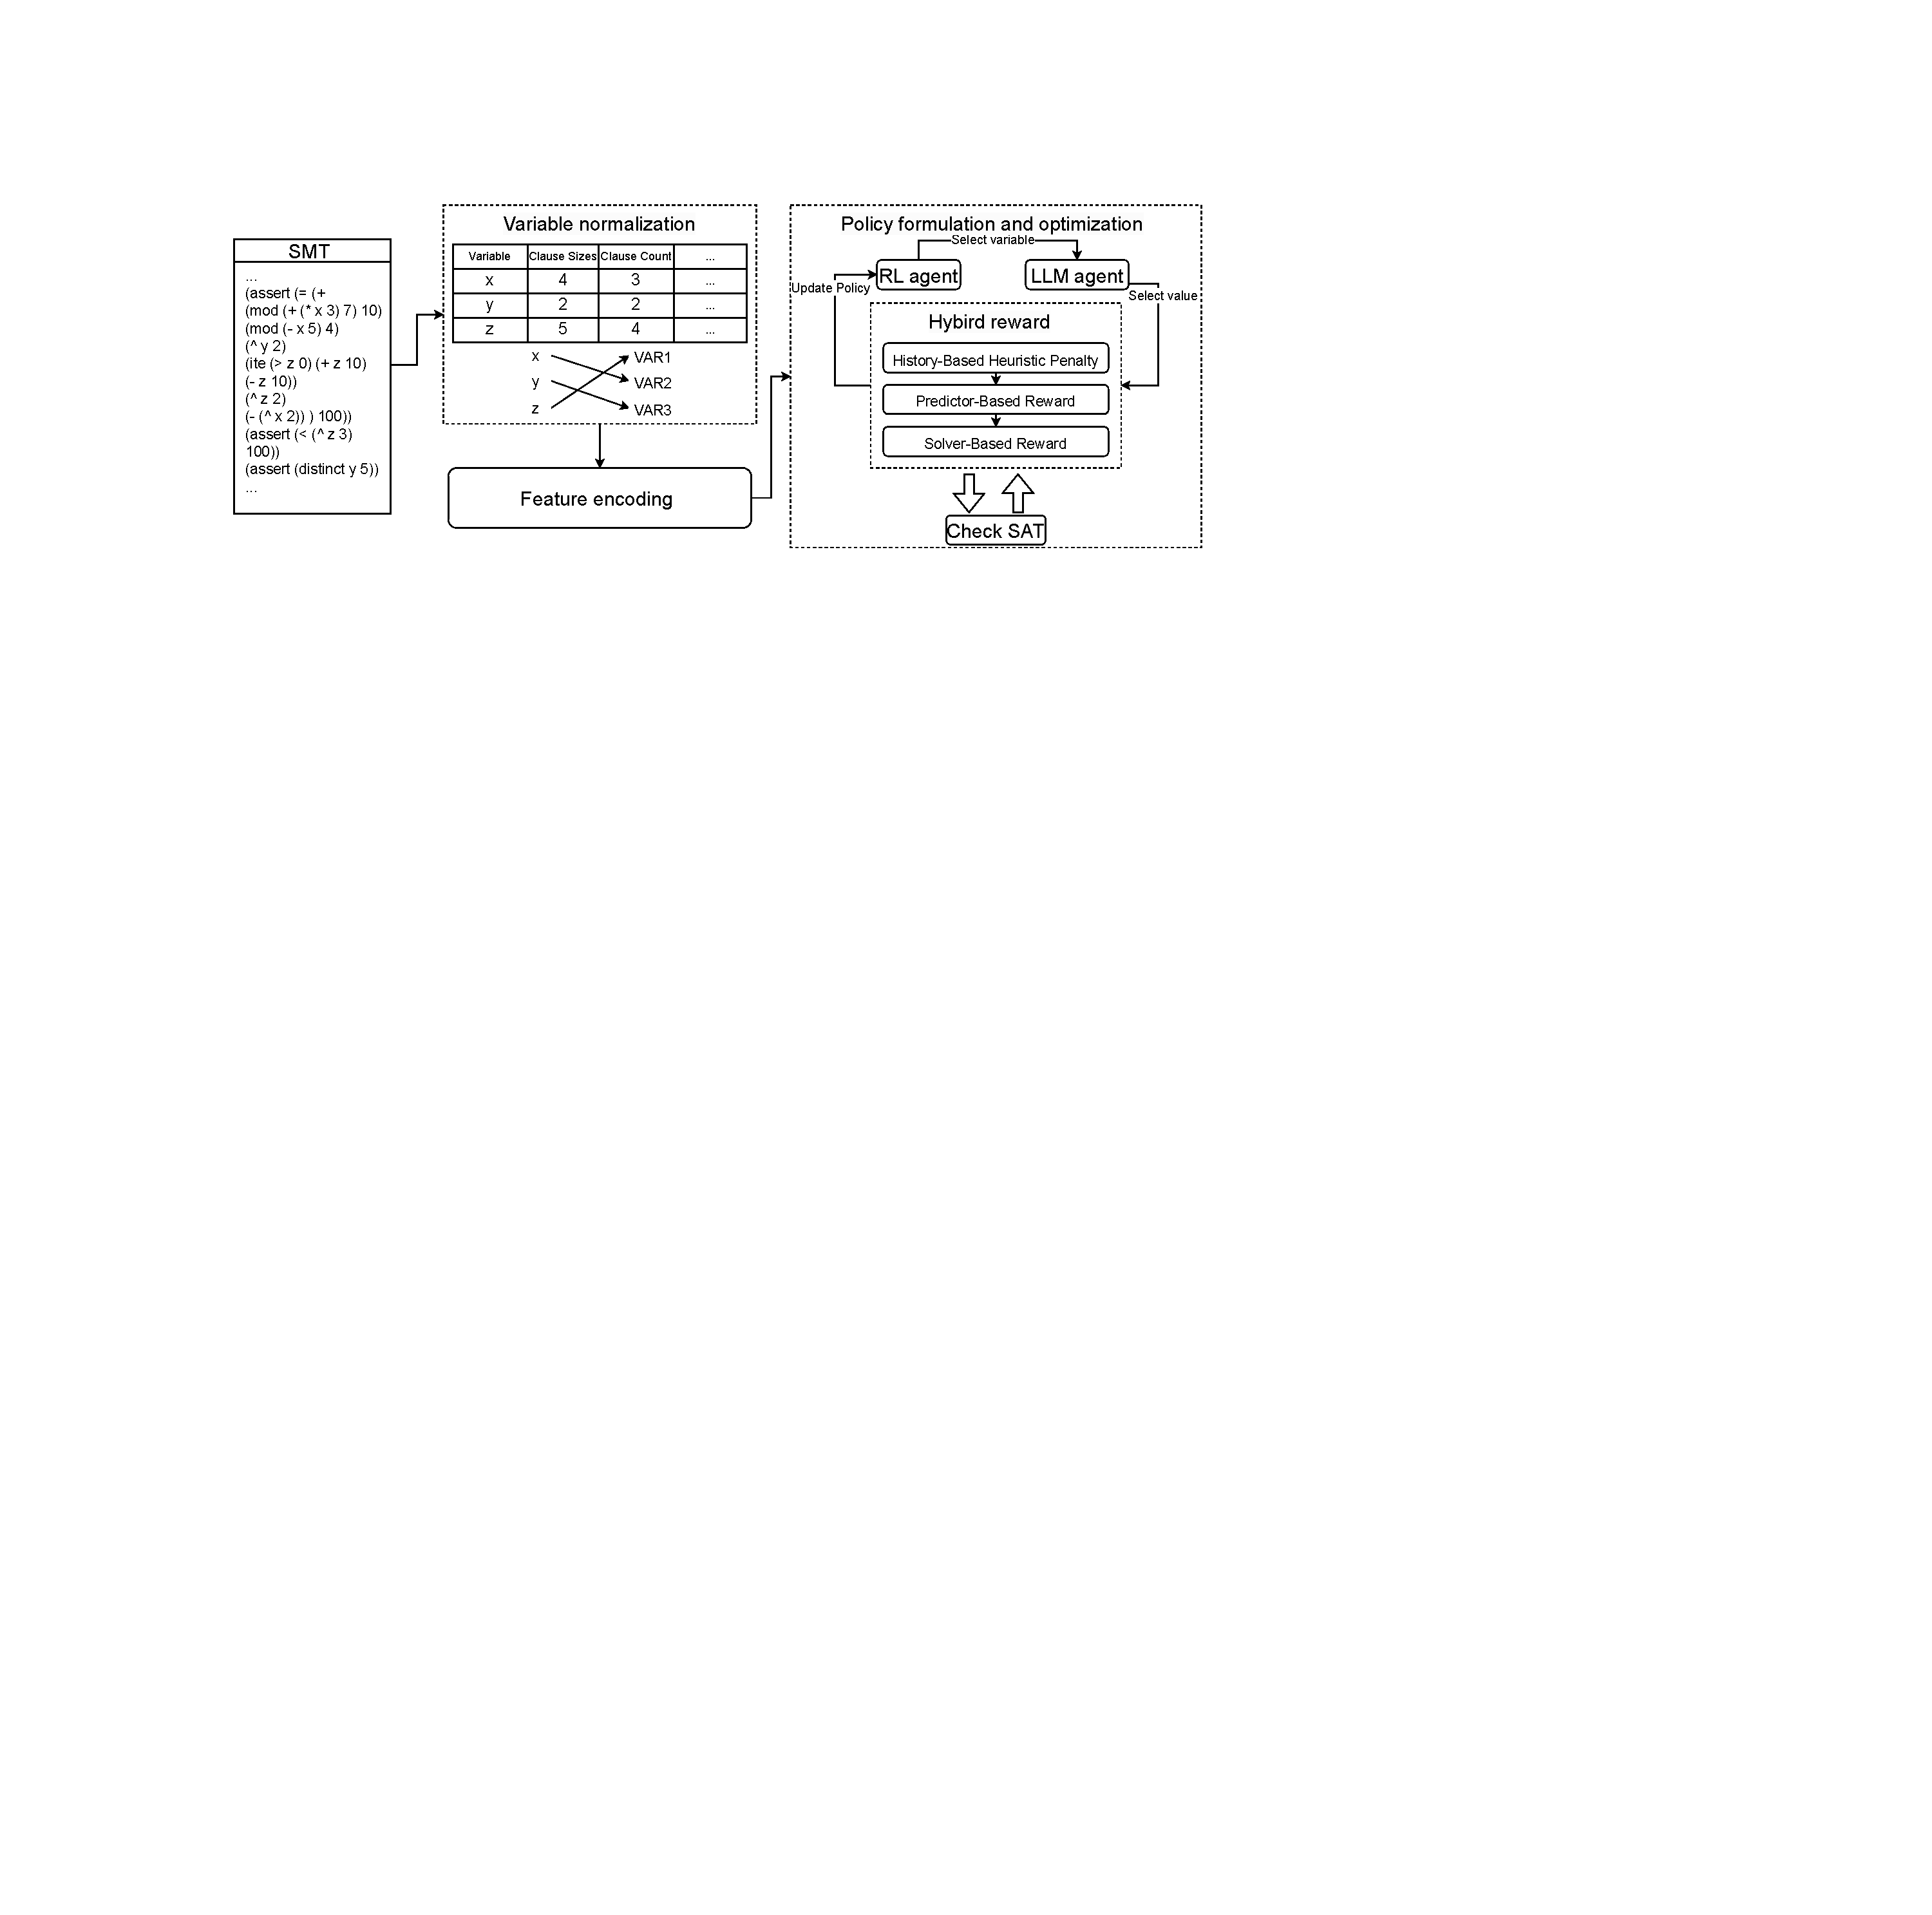
\includegraphics[width=\linewidth]{pics/method.pdf}
    \caption{Workflow of \tool{}.}
    \label{fig:method}
\end{figure}

Figure~\ref{fig:method} illustrates the architecture of \tool{}， which consists of four components: variable normalization, feature encoding, hybrid reward system, and dual-agent simplification policy.
% \wyc{use the following: Figure~\ref{fig:method} illustrates the architecture of \tool{}, which consists of xxx components: xxx, xxx, xxx. 
% Then, use what you have written, \ie, The process begins with...} \wyc{The components you introduced must be consistent with that in the workflow.}
The process begins with variable normalization which creates a consistent foundation for learning. To ensure our models can generalize across formulas that are structurally identical but use different variable names, this stage canonicalizes the input by sorting variables based on a stable vector of their structural attributes, yielding a permutation-invariant representation for the agent.

The canonical formula is then transformed into a state representation by our feature encoding component. This component converts the symbolic text into a high-dimensional vector designed to capture the formula's underlying structure. This vector serves two primary purposes. First, it provides the contextual input required for the \RL{} agent's policy decisions. Second, it is used to train two predictive models: a classifier to estimate a formula's solvability and another to predict its solving time.  As we will see, these pre-trained predictors are crucial for guiding the agent's learning.

To guide the learning process effectively, we then designed a hybrid reward system. Recognizing that feedback in the \SMT{} environment is inherently sparse and expensive, this system provides a rich learning signal by combining sparse but definitive outcomes from the \SMT{} solver, dense heuristic guidance from pre-trained predictive models, and history-based penalties to prune the search space.

Finally, guided by this rich reward signal, the heart of our approach is the dual-agent architecture. This architecture is designed to address the challenge of learning over the environment's vast, composite discrete action space, where a complete action consists of both a variable and a value. Instead of learning a single, monolithic policy to navigate this space, our solution decomposes the decision-making process into two complementary roles. A strategic \RL{} agent learns a policy to select what to simplify (variable selection), effectively deciding which dimension of the action space to explore. Subsequently, a tactical \LLM{} uses its semantic reasoning capabilities to propose \textit{how} to simplify (value generation), completing the action pair. This division of labor allows each component to leverage its unique strengths---the RL agent for long-term, feedback-driven planning and the LLM for rich, context-aware reasoning.


\subsection{Variable Normalization}
\label{sec:normalization}
\wyc{This subsection seems not clear to me. The method should be explained more clear (discuss steps first, then explain the benefit.). \eg, adding examples. Second, the design choice is missing (\eg, why do you use the canonicalization method). Finally, why does this method work?}

A foundational challenge for applying machine learning methods to symbolic formulas is input variance~\cite{zaheer2017deep,battaglia2018relational}: two structurally isomorphic formulas may be textually distinct due to arbitrary variable naming, which prevents a learned model from generalizing. To overcome this, \tool{} begins with a deterministic canonicalization of the input SMT formula. The goal of this process is to standardize the naming and ordering of variables based on their structural roles, ensuring that any two structurally equivalent formulas are mapped to the exact same textual representation. This allows our learning models to focus on the underlying semantic structure rather than superficial naming conventions.

\subsubsection{Canonicalization via Structural Sorting}
The core of this process is a deterministic sorting process that reorders variables based on their structural importance. For each variable, we first extract a vector of numerical attributes that serve as proxies for its influence within the formula. These attributes, detailed in Table~\ref{tab:normalization-attributes}, are arranged in a predefined order of importance, including metrics like the total size of clauses a variable appears in, its frequency, and the number of distinct clauses it participates in.
The sorting itself is performed using this ordered vector of attributes. Specifically, all variables are first sorted according to the most important attribute (\ie, `Variable clause sizes'). Any ties among variables are then resolved by sorting them according to the second most important attribute (`Variable to clause count'), and this tie-breaking process continues sequentially down the entire attribute list. This stable, multi-level sorting procedure guarantees that a unique and deterministic ordering is produced for any given formula. Finally, the sorted variables are systematically renamed to a canonical form, such as $\mathit{VAR}_1, \dots, \mathit{VAR}_n$, completing the canonicalization.

\subsubsection{Impact on Policy Learning}
A simpler approach, like alphabetical sorting, would be brittle and fail to capture any structural information. In contrast, our chosen attributes act as robust proxies for a variable's semantic importance, a principle that aligns with feature engineering for code analysis~\cite{henkel2023neural}. By encoding this importance into the variable ordering, we create a representation that is not only consistent but also informative for the downstream agent. This method is effective because it makes the learning models invariant to superficial syntactic differences, a crucial step when applying machine learning to source code~\cite{alon2019code2vec}. This process significantly reduces the variance of the state space the \RL{} agent must explore~\cite{bengio2009learning}, provides a stable action space where an action consistently targets a variable of similar structural importance, greatly simplifying the policy learning challenge~\cite{laskin2021urlb}.
\begin{table}[!t]
    \centering
    \caption{Attributes for variable normalization, ordered by importance.}
    \label{tab:normalization-attributes}
    \begin{tabular}{@{} l p{0.72\linewidth} @{} }
    \toprule
        \multicolumn{1}{c}{\textbf{Attribute}} & \multicolumn{1}{c}{\textbf{Description}} \\ \midrule
        Variable clause sizes   & The sum of elements in clauses where the variable appears. \\ 
        Variable to clause count & The number of distinct clauses the variable appears in. \\ 
        Variable frequencies & The total number of times the variable occurs in the formula. \\ 
        Total logic operations & The number of logical operations the variable participates in. \\ 
        Variable constant interactions & The count of clauses where the variable appears with a constant. \\ \bottomrule
    \end{tabular}
\end{table}
\subsection{Feature Encoding}\lz{introduce "what" in overview, introduce "why" in this section with short explanation}
\label{sec:feature-encoding}
To enable an \RL{} agent to make informed decisions, the \SMT{} formula must be transformed into a rich, machine-readable state representation. It is well-established that purely syntactic representations often fail to capture the complex semantic relationships within structured code or logical formulas, limiting the generalization capabilities of learning models~\cite{alon2019code2vec}. We therefore employ a \PLM{} to serve as our feature encoder, a technique that has proven highly effective for generating deep, contextualized representations of source code~\cite{feng2020codebert}.

% To enable the \RL{} agent to make informed decisions, the SMT formula must be transformed into a machine-readable state representation that captures its underlying semantic properties. While purely syntactic representations often fail to capture such complex relationships and thus limit model generalization~\cite{alon2019code2vec}, pre-trained language models (PLMs) have proven highly effective for generating deep, contextualized representations of structured text like source code~\cite{feng2020codebert}. We therefore employ a PLM-based feature encoder. Unlike handcrafted feature engineering, which would be brittle and difficult to scale across different SMT logics, this approach allows for the automatic learning of semantic nuances directly from data. The entire normalized SMT formula is provided as input to the encoder, which produces a holistic, fixed-size vector embedding to serve as the complete state representation, $s_t$, for the \RL{} agent.


% The encoding process leverages the PLM's ability to comprehend structured text. The entire normalized \SMT{} formula is provided as input to the model, which processes it to produce a holistic, fixed-size vector embedding. This vector is designed to capture the rich semantic relationships and overall structure of the constraints, serving as the complete state representation, $s_t$, for the \RL{} agent at timestep $t$.

% The design rationale behind using a PLM is its ability to learn effective feature hierarchies automatically from data, a core principle of deep learning~\cite{bengio2013representation}. Unlike handcrafted feature engineering, which would be brittle and difficult to scale across different \SMT{} logics, a PLM can automatically learn to capture the semantic nuances of operators, the relationships between variables, and the overall structure of the formula. This method is effective because it provides the \RL{} agent with a dense, semantic state that implicitly encodes much of the information an expert might use for reasoning. A high-quality state representation is fundamental to an agent's ability to learn a non-trivial and generalizable policy, especially in complex domains where such representations can make the learning problem significantly more tractable~\cite{sutton2018reinforcement}.

\subsection{The Hybrid Reward System}
\label{sec:reward-system}

Effective policy learning in \RL{} hinges on receiving frequent and informative feedback. However, the SMT solving environment presents two fundamental challenges for reward design. First, the SMT solver is a well-known performance bottleneck~\cite{cadar2013symbolic}; relying solely on its ground-truth outcomes would require invoking it after every action, rendering the learning process computationally intractable. Second, the environment's rewards are naturally sparse. An agent may perform a long sequence of simplification actions before receiving a definitive outcome, a classic challenge in \RL{} known as the temporal credit assignment problem~\cite{sutton2018reinforcement}.

To overcome these challenges, we designed a hybrid reward system that synergistically combines signals from two distinct real-time sources---the solver and a set of predictive models---and augments them with a history-based heuristic penalty. Crucially, to balance the trade-off between signal density and computational cost, the system employs a partial evaluation strategy, where feedback is periodically generated from a random subset of the formula's constraints rather than the entire set.

\subsubsection{Solver-Based Reward}
The most definitive feedback originates from the SMT solver, providing a high-fidelity, ground-truth signal. The solver's primary role is to provide the ultimate reward through a comprehensive check on the entire formula, typically triggered once at the end of an episode. This anchors the policy to the true objective but is inherently sparse. To enrich the learning process with more frequent feedback, we also employ the solver strategically for partial evaluations. These lightweight checks involve invoking the solver with a short timeout on a subset of constraints, from which a quick \texttt{unsat} result yields a medium-fidelity negative reward, enabling efficient pruning of the search space at a much lower computational cost.

\subsubsection{Predictor-Based Reward}
Complementing the solver, our pre-trained predictive models offer a continuous stream of low-cost, dense guidance. Specifically, we employ two distinct neural network models: a binary classifier, $P_{solve}$, that predicts the likelihood of a formula being satisfiable, and a multi-class classifier, $P_{time}$, that estimates the solving time by assigning it to a predefined complexity bucket.

To ensure the integrity of our evaluation and prevent any data leakage, these predictors are trained on a separate partition of the data. For each benchmark dataset used in our experiments, we perform a strict 50/50 split: one half is used exclusively for training $P_{solve}$ and $P_{time}$, while the other half is reserved as the test set for our online simplification agent. 

During the simplification process, these lightweight models provide the reward signal in two primary ways. They are tightly integrated with our partial evaluation strategy, where they are queried on the same constraint subset as the solver to provide an immediate estimate of progress. Furthermore, their low computational cost allows them to be queried on the full formula at any step, ensuring a constant stream of moment-to-moment feedback. This dense signal directly mitigates the temporal credit assignment problem and provides a smooth learning gradient for the agent.


\subsubsection{History-Based Heuristic Penalty}
In addition to the two real-time reward sources, our system incorporates an orthogonal component that leverages the agent's past experience: a history-based heuristic penalty. This mechanism functions as a form of agent memory, utilizing a repository of counterexamples that stores previously failed action sequences. If the agent's current action sequence matches a known failing path, a significant negative penalty is immediately applied. This low-cost lookup operation acts as an efficient search-space pruning mechanism and provides a deterministic penalty for repeated mistakes, thereby accelerating policy convergence.

\subsubsection{Synergy}
The final reward signal $r_t$ is a synergistic composition of these components. The definitive but sparse signals from full solver evaluations ensure the policy converges towards the true objective. Meanwhile, the combination of denser feedback from partial solver checks and continuous heuristic guidance from the predictors provides a rich gradient for exploration. Finally, the history-based penalty leverages memory to efficiently prune the search space. Together, they form a robust and efficient hybrid reward function capable of guiding the agent through the challenging landscape of SMT constraint simplification.

\subsection{Dual-Agent Architecture}
\label{sec:policy-formulation-and-optimization}

To learn an effective simplification strategy, we formalize the task as a \MDP{} and train a \RL{} agent. The agent's goal is to learn a policy, $\pi(a_t|s_t)$, that maps a given formula state to a simplification action that maximizes the expected long-term reward.
This section details our complete \MDP{} formulation by defining its core components---the state representation ($s_t$), the action space ($a_t$), and the hybrid reward ($r_t$)---and concludes by detailing the approach for optimizing the agent's policy.

\subsubsection{State Representation}
The agent's decision at each timestep is conditioned on the current state of the formula, $s_t$. As defined in Section~\ref{sec:feature-encoding}, we use the high-dimensional vector embedding produced by a \PLM{} as the state representation. This vector captures the rich semantic and structural properties of the canonicalized formula, providing the necessary context for the policy.

\subsubsection{Action Space and Dual-Agent Design}
The action space for simplification is a complex, hybrid domain $\mathcal{A} = \mathcal{V} \times \mathcal{C}$, where $\mathcal{V}$ is the finite, discrete set of canonical variables, and $\mathcal{C}$ is the virtually infinite set of possible integer values. A single RL agent cannot tractably learn a policy over this joint space.
Our core contribution is to decompose this action into two sequential sub-problems, governed by the principle of task decomposition based on the core strengths of each component\cite{kautz2022third}. The high-level, strategic decision of \textit{what} variable to simplify is assigned to an RL agent, whose policy operates over the finite space $\mathcal{V}$. Conversely, the low-level, tactical decision of \textit{how} to simplify is delegated to a pre-trained LLM. Conditioned on the state and the chosen variable, the LLM generates a contextually plausible value. This is achieved by providing it with a carefully constructed prompt that includes the full formula context, the target variable, and a list of previously failed values (counterexamples) to steer it away from known unsuccessful attempts, as shown in Figure~\ref{fig:prompt}. 
A key consequence of this design is that only the RL agent undergoes online, gradient-based policy updates, while the LLM remains a static, pre-trained model with frozen parameters, adapting only through the in-context information provided in the prompt. This paradigm of pairing a dynamic, learning policy with a static, pre-trained model has proven effective for training large models with reinforcement learning. For instance, Ouyang \etal~\cite{ouyang2022training} use a frozen reference model to regularize the policy during optimization, ensuring its core capabilities are preserved. In our framework, the LLM serves as a stable source of general semantic knowledge, while the RL agent specializes in learning a policy for the specific task of SMT simplification.
This is intentional, as it preserves the specialization of each agent. The \RL{} agent's role is to adapt and learn a domain-specific strategy, while the LLM's role is to serve as a stable source of general semantic knowledge. Attempting to fine-tune the LLM on the sparse and noisy reward signal from the solver would risk catastrophically degrading its valuable pre-trained abilities and would be computationally infeasible. While the LLM does not learn via gradients, it does adapt within an episode through in-context learning: by incorporating previously failed values into its prompt as counterexamples, it is steered away from known unpromising suggestions.

\subsubsection{Hybrid Reward}
To guide the agent's learning, we use the multi-level hybrid reward system detailed in Section~\ref{sec:reward-system}. The final reward, $r_t$, for taking a complete action $a_t = (v_t, c_t)$ is a composite signal combining sparse, ground-truth feedback from the solver with dense, estimated rewards from our predictive models. This hybrid reward is crucial for mitigating the credit assignment problem. We emphasize that the LLM is part of the action-generation process, not the reward-generation process.

\subsubsection{Policy Optimization via Soft Actor-Critic}
We learn the variable selection policy $\pi$ using \SAC{}~\cite{haarnoja2018soft}, an off-policy actor-critic method based on the maximum entropy framework. Its selection is principally motivated by two features that directly address the challenges of SMT constraint simplification. First, interacting with the environment is computationally expensive due to the cost of SMT solver invocations. As an off-policy method that leverages a replay buffer, \SAC{} is highly sample-efficient, making it well-suited for learning in environments where data collection is costly~\cite{levine2020offline}. Second, the space of effective simplification strategies is vast and requires extensive exploration to avoid converging to a suboptimal policy. The core mechanism of SAC, entropy maximization, encourages robust exploration by incentivizing the agent to act as randomly as possible while still accomplishing its objective, a critical feature for complex decision-making problems~\cite{haarnoja2018soft}. The \SAC{} agent consists of an actor network, which models the policy, and critic networks, which estimate the expected future rewards. The learning process follows a standard online RL loop. At each step, the agent observes state $s_t$, selects a variable $v_t$, the LLM proposes a value $c_t$, and the environment returns the hybrid reward $r_t$ and the next state $s_{t+1}$. This transition $(s_t, v_t, r_t, s_{t+1})$ is stored in a replay buffer. The agent is then trained by sampling mini-batches from this buffer to update its actor and critic networks, progressively improving its policy to maximize the expected cumulative reward.

\begin{figure}[!t]
    \centering
    \label{fig:prompt}
    \Description{An example of the prompt structure used to query the Large Language Model for value suggestions, including context from the SMT formula.}
    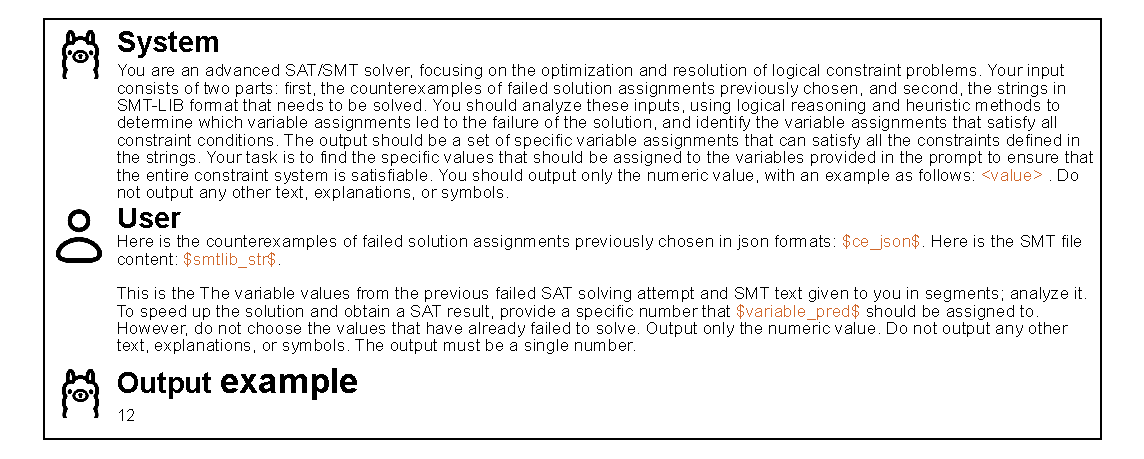
\includegraphics[width=\textwidth,trim=0 8pt 0 8pt,clip]{pics/prompt.pdf}
    \caption{Prompt template for heuristic value generation by the LLM.}
\end{figure}

% \wyc{"Overall Algorithm" seems to be a better title of the subsection}

% \wyc{give the high-level idea of the algorithm (\eg, explain the alg using three major steps), then explain the algorithm line by line.}

% The individual components of our methodology are orchestrated by a single, closed-loop algorithm that operationalizes our framework. As detailed in Algorithm~\ref{alg:main}, this procedure follows a strategic, trial-and-error exploration process, structured as a nested loop. The outer loop initiates new simplification attempts, or "trials," while the inner loop extends the current simplification sequence step-by-step. This process synergistically integrates the components detailed previously: the algorithm is initialized using our variable normalization and feature encoding schemes; the inner loop is driven by the dual-agent policy; and the agent's learning is guided by the multi-level hybrid reward system. A key innovation of this process is a performance-monitoring mechanism that uses our predictive models to greedily extend promising simplification paths, while quickly abandoning and learning from those that degrade performance.

% The algorithm begins by preparing the necessary components for a given formula, $Q_{init}$ (Lines~\ref{alg:line:normalize}--\ref{alg:line:init-history}). This involves applying our variable normalization process (Section~\ref{sec:normalization}) to the initial formula and initializing the SAC agent and the history of counterexamples. The outer loop (Line~\ref{alg:line:outer-loop}) then manages the overall simplification process under a global time budget, initiating new trials as needed.

% Each trial starts by resetting the environment to the original, canonicalized formula, $Q_{base}$ (Line~\ref{alg:line:trial-reset}). The feature encoding component (Section~\ref{sec:feature-encoding}) is invoked to generate the initial state embedding, $s$, and a baseline performance score, $last\_perf$, is initialized to zero (Line~\ref{alg:line:perf-init}). This provides a neutral starting point for performance comparison throughout the trial. The inner loop (Line~\ref{alg:line:inner-loop}) then begins to extend the current simplification sequence. At each step, the dual-agent policy (Section~\ref{sec:policy-formulation-and-optimization}) is executed: the RL agent selects a variable $v_t$, and the LLM proposes a value $c_t$ based on the accumulated counter-examples from previous failed trials (Lines~\ref{alg:line:select-var}--\ref{alg:line:propose-val}).

% After the formula is simplified, the framework evaluates the new state. The feature encoder is re-invoked to produce the next state embedding $s'$ (Line~\ref{alg:line:embed-next}), and the backend solver attempts to solve the modified formula. The multi-level hybrid reward computation simultaneously evaluates both the reward signal and a performance score, $current\_perf$, based on predictive model outputs and solver results (Line~\ref{alg:line:compute-reward}). This performance check is the primary driver of the exploration strategy. If the score degrades compared to the baseline (Line~\ref{alg:line:reset-cond}), the current trial is deemed a failure. The failing sequence is recorded (Line~\ref{alg:line:add-history}), and the inner loop terminates, triggering a new trial. Otherwise, the agent's policy is updated using the full multi-level hybrid reward (Line~\ref{alg:line:compute-reward}), as detailed in Section~\ref{sec:reward-system}, and the state is advanced for the next iteration (Line~\ref{alg:line:advance-state}).

\subsection{Overall Algorithm}
\label{sec:algorithm}
\wyc{"Overall Algorithm" seems to be a better title of the subsection}

\wyc{give the high-level idea of the algorithm (\eg, explain the alg using three major steps), then explain the algorithm line by line.}
The individual components of our methodology are orchestrated by the \tool algorithm, a single, closed-loop procedure that operationalizes our framework, as detailed in Algorithm~\ref{alg:main}. The algorithm follows a strategic, trial-and-error exploration process structured as a nested loop: an outer loop initiates new simplification attempts (``trials''), while an inner loop extends the current simplification sequence step-by-step. A key innovation guiding this process is a performance-monitoring mechanism that defines the ``error'' phase of this exploration: it uses our predictive models to greedily pursue promising paths while quickly abandoning those that degrade performance. These abandoned sequences are treated as learning opportunities---``errors''---and are recorded as counterexamples to inform subsequent trials. The process begins by preparing the initial formula $Q_{init}$ through variable normalization and initializing the \SAC{} agent and the repository for these counterexamples (Lines~\ref{alg:line:normalize}--\ref{alg:line:init-history}). The outer loop then manages the overall simplification process, launching new trials until a satisfying assignment is found or an external termination condition (\eg, a timeout) is met (Line~\ref{alg:line:outer-loop}).

Each trial starts by resetting the environment to the original, canonicalized formula, $Q_{base}$ (Line~\ref{alg:line:trial-reset}). The feature encoding component (Section~\ref{sec:feature-encoding}) is invoked to generate the initial state embedding, $s$, and a baseline performance score, $last\_perf$, is initialized to zero (Line~\ref{alg:line:perf-init}). This provides a neutral starting point for performance comparison throughout the trial. The inner loop (Line~\ref{alg:line:inner-loop}) then begins to extend the current simplification sequence. At each step, the dual-agent policy (Section~\ref{sec:policy-formulation-and-optimization}) is executed: the RL agent selects a variable $v_t$, and the LLM proposes a value $c_t$ based on the accumulated counter-examples from previous failed trials (Lines~\ref{alg:line:select-var}--\ref{alg:line:propose-val}).

After the formula is simplified, the framework evaluates the new state. The feature encoder is re-invoked to produce the next state embedding $s'$ (Line~\ref{alg:line:embed-next}), and the backend solver attempts to solve the modified formula. The multi-level hybrid reward computation simultaneously evaluates both the reward signal and a performance score, $current\_perf$, based on predictive model outputs and solver results (Line~\ref{alg:line:compute-reward}). This performance check is the primary driver of the exploration strategy. If the score degrades compared to the baseline (Line~\ref{alg:line:reset-cond}), the current trial is deemed a failure. The failing sequence is recorded (Line~\ref{alg:line:add-history}), and the inner loop terminates, triggering a new trial. Otherwise, the agent's policy is updated using the full multi-level hybrid reward (Line~\ref{alg:line:compute-reward}), as detailed in Section~\ref{sec:reward-system}, and the state is advanced for the next iteration (Line~\ref{alg:line:advance-state}).

\begin{algorithm}[!t]
\caption{The COMPASS Simplification Algorithm with Performance-Monitored Exploration}
\label{alg:main}
\raggedright\textbf{Input:} $Q_{init}$ - initial SMT constraint formula; $S$ - backend SMT solver
\begin{algorithmic}[1]
\Procedure{SimplifyConstraint}{$Q_{init}, S$}
    \State $Q_{base} \gets \Call{Normalize}{Q_{init}}$ \label{alg:line:normalize}
    \State $agent \gets \Call{InitializeSAC}{\Call{GetActionSpaceSize}{Q_{base}}}$
    \State $counter\_ex \gets [\,]$ \Comment{Stores all discovered failing sequences} \label{alg:line:init-history}
    \While{True} \Comment{Outer Loop: Manages new trials until solution or termination} \label{alg:line:outer-loop}
        \State $Q \gets Q_{base}$; $s \gets \Call{Embed}{Q}$ \label{alg:line:trial-reset}
        \State $last\_perf \gets 0$ \Comment{Initialize performance baseline for the trial} \label{alg:line:perf-init}
        \State $current\_sequence \gets [\,]$
        \While{True} \Comment{Inner Loop: Extends the current simplification sequence} \label{alg:line:inner-loop}
            \State $v_t \gets agent.\Call{SelectVariable}{s}$ \label{alg:line:select-var}
            \State $c_t \gets \Call{LlmProposeValue}{Q, v_t, counter\_ex}$ \label{alg:line:propose-val}
            \State $Q' \gets \Call{Concretize}{Q, v_t, c_t}$
            \State $current\_sequence.\Call{append}{(v_t, c_t)}$
            \State $s' \gets \Call{Embed}{Q'}$ \label{alg:line:embed-next}
            \State $(res, t_{solve}) \gets S.\Call{solve}{Q', \Call{GetAdaptiveTimeout}{s'}}$
            
            \State $(r, current\_perf) \gets \Call{ComputeHybridReward}{res, t_{solve}, s, s', counter\_ex}$ \label{alg:line:compute-reward}
            \State $agent.\Call{Update}{s, v_t, r, s'}$
            
            \If{$current\_perf < last\_perf$} \label{alg:line:reset-cond}
                \State $\Call{AppendToHistory}{counter\_ex, current\_sequence}$ \Comment{Record failing sequence} \label{alg:line:add-history}
                \State \textbf{break} \Comment{End this trial and start a new one}
            \ElsIf{$res = \texttt{sat}$}
                \State \Return $\langle \texttt{sat}, \Call{GetModel}{S} \rangle$
            \EndIf
            \State $s \gets s'$; $Q \gets Q'$; $last\_perf \gets current\_perf$ \Comment{Advance to the next step} \label{alg:line:advance-state}
        \EndWhile
    \EndWhile
    \State \Return $\langle \text{unknown} \rangle$
\EndProcedure
\end{algorithmic}
\end{algorithm}

\section{EVALUATION}
\label{sec:evaluation}
% This section empirically evaluates our AI-assisted framework, \tool. We designed experiments to assess its effectiveness on challenging problems, the scalability of its learned policies, and the synergy between its \RL{} and \LLM{} components.
This section empirically evaluates our framework, \tool{}. We designed our experiments to answer three core research questions that progressively validate our approach, moving from overall effectiveness to internal component analysis and finally to practical deployment.

\subsection{Research Questions}
Our evaluation aims to answer the following research questions:
\begin{enumerate}[leftmargin=*,label=\textbf{RQ\arabic*.},wide, labelwidth=!, labelindent=0pt]
    \item \textbf{Effectiveness of \tool{}.} How effective is \tool{} across different constraint types, and SMT solver architectures?

    \item \textbf{Ablation Study of \tool{}.} What are the individual contributions of the \RL{} and \LLM{} components, and how do different \LLM{}s affect overall performance?
    
    \item \textbf{Effectiveness of Selective Simplification.} Does a selective simplification strategy for the \tool{} improve the overall trade-off between performance and computational cost compared to a non-selective approach?
\end{enumerate}

Our evaluation is designed to provide a comprehensive validation of \tool{}. We begin by addressing the foundational questions of overall effectiveness (\textbf{RQ1}) and the synergistic contributions of the core components through ablation studies (\textbf{RQ2}). Building on this foundation, \textbf{RQ3} addresses the challenge of practical deployment. While \tool{} is powerful, its AI-driven process introduces computational overhead compared to direct solving. Naively applying this expensive simplification to every incoming constraint would be inefficient, potentially slowing down the overall system on simpler problems where it is not needed. Therefore, a mechanism to selectively apply it only to genuinely difficult cases is essential. RQ3 is thus designed to investigate this practical trade-off, determining whether the performance benefits gained by applying \tool{} to hard problems can justify and outweigh the computational overhead introduced by the guidance mechanism itself.




\subsection{Experimental Setup}

\subsubsection{Implementation.} Our implementation is built upon the Pearl framework\footnote{https://github.com/facebookresearch/Pearl} and utilizes Ollama\footnote{https://github.com/ollama/ollama} for language model hosting. % Added code scale information in response to wyc's comment.
The complete implementation comprises approximately 20,150 lines of Python code for core experimental functionality, including constraint solving orchestration, multi-solver integration, experimental evaluation framework, and data processing utilities.

\subsubsection{Benchmarks.} Our evaluation is conducted on two distinct benchmarks: SMTimer\cite{luoBoostingSymbolicExecutionTime2021}, which contains program-derived constraints from Coreutils\footnote{https://www.gnu.org/software/coreutils/}, BusyBox\footnote{https://busybox.net/}, angr\footnote{https://angr.io/}, and KLEE, and the public \SMTCOMP{}\footnote{https://smt-comp.github.io/2024/} benchmarks, which we use to assess scalability against harder, multi-theory constraints\cite{BST10,klee,mechtaevSemanticProgramRepair2018}. To ensure a fair and meaningful comparison, we apply a consistent preprocessing pipeline to these datasets. This involves: (i) excluding trivially solvable instances where the baseline solver takes 300 seconds or less, as well as all \texttt{unsat} cases; (ii) focusing on problems with more than five variables ($|V|>5$) to provide a sufficiently complex action space for the RL agent; and (iii) enforcing uniform timeouts and normalizing solver status codes. Using the processed SMTimer data, we train two predictive models (for solvability and time-bucket classification) on textual features extracted from the SMT-LIB2 formulas, with further hyperparameter details provided in the appendix. 

% \subsubsection{Hardware.} All experiments were executed on a desktop workstation equipped with an Intel\textsuperscript{\textregistered} Core\texttrademark{} i7-11700K CPU, 128 GB of RAM, and an NVIDIA GeForce RTX 3080 Ti GPU, running Ubuntu 20.04 LTS. 
% The LLM service was hosted in a Docker container on a separate, high-performance server equipped with AMD EPYC 9654 96-Core, 1.5 TiB of RAM and NVIDIA H800 PCIe GPU. 

% \subsubsection{Language Models.} % Clearly specified LLM models used in response to wyc's inquiry.
% We evaluate three state-of-the-art large language models: LLaMA 3.1:70B, LLaMA 3.3:70B, and DeepSeek-R1:70B. All models are hosted via Ollama with consistent temperature settings (0.7) and maximum token limits (2048) to ensure reproducible results across experiments.
\subsubsection{Hardware and Models}
All experiments were executed on a desktop workstation equipped with an Intel\textsuperscript{\textregistered} Core\texttrademark{} i7-11700K CPU, 128 GB of RAM, and an NVIDIA GeForce RTX 3080 Ti GPU, running Ubuntu 20.04 LTS. 
The \LLM{} service was hosted in a Docker container on a separate, high-performance server equipped with AMD EPYC 9654 96-Core, 1.5 TiB of RAM and NVIDIA H800 PCIe GPU. 
We evaluate three 70-billion-parameter \LLM{}s: LLaMA 3.1, LLaMA 3.3, and DeepSeek-R1. All models were obtained from the official Ollama library using their respective 70B tags (\eg{}, \texttt{ollama pull llama3.1:70b}). The on-disk size for each model is approximately 43GB, which corresponds to a 4-bit quantized version (\eg{}, Q4\_K\_M). 
% This quantization level provides a strong balance between computational efficiency and reasoning performance. To ensure reproducible results, all models are queried via Ollama with a consistent temperature setting of 0.7 and a maximum token limit of 2048.



\subsection{RQ1: Effectiveness of \tool}
\label{sec:rq1-effectiveness}

% Restructured RQ1 as comprehensive effectiveness evaluation, integrating original RQ1/RQ2/RQ4 content, organized in logical sequence "SMTimer baseline validation → SMT-COMP scalability → multi-solver generalization" to provide more complete and coherent effectiveness evidence.

\subsubsection{Results on SMTimer}

% Restructured RQ1 to provide comprehensive effectiveness evaluation by integrating multi-solver comparison (original Table 4) with Z3-specific analysis (original Table 2), followed by detailed case study analysis.
To verify the effectiveness of our method, we conducted experiments on the SMTimer dataset across multiple SMT solvers. % Clarified timeout settings with SMT-COMP standard reference; rewrote constraint filtering logic for clearer expression; added SMT-COMP timeout standard footnote link.
Following SMT-COMP's standard configuration\footnote{SMT-COMP 2024 uses 1200-second timeouts: \url{https://smt-comp.github.io/2024/rules.html}}, we set a 1200-second timeout and consider a constraint ``solved'' if the solver returns \texttt{sat} within the time limit; timeouts are treated as \texttt{unknown}. 
We exclude constraints with baseline solving times below 300 seconds, since simpler cases can be efficiently solved without additional simplification. We also restricted our experiments to constraints with more than 5 variables, as the RL agent requires sufficient action space for meaningful strategy exploration.

\begin{table}[t]
\captionsetup{skip=1pt}
\centering
\caption{Multi-Solver Performance Comparison on SMTimer Dataset. Here, "+" denotes applying \tool as a preprocessing layer to the baseline solver.}
\label{tab:multi-solver-comparison}
\begingroup
\setlength{\tabcolsep}{4pt}% tighter columns
\renewcommand{\arraystretch}{0.9}% tighter rows
\normalsize
\begin{tabular}{lccccccc}
\toprule
\multirow{2}{*}{Solver} & \multirow{2}{*}{Total} & \multicolumn{2}{c}{Solved Constraints} & \multicolumn{2}{c}{Success Rate (\%)} & \multicolumn{2}{c}{Avg. Time (s)} \\
\cmidrule(lr){3-4} \cmidrule(lr){5-6} \cmidrule(lr){7-8}
& & Baseline & +\tool & Baseline & +\tool & Baseline & +\tool \\
\midrule
Z3 & 337 & 72 & 94 & 21.4 & 27.9 & 561 & 214 \\
CVC5 & 555 & 113 & 357 & 20.4 & 64.3 & 1059 & 347 \\
BVParti & 33 & 2 & 19 & 6.1 & 57.6 & 694 & 100 \\
MathSAT & 150 & 29 & 100 & 19.3 & 66.7 & 757 & 450 \\
\bottomrule
\end{tabular}
\endgroup
\end{table}

To evaluate the portability of our framework, we test it on four SOTA solvers with diverse architectures: the widely-used general-purpose solvers Z3~\cite{demoura2008z3} and CVC5~\cite{cvc5}; the arithmetic-focused solver MathSAT~\cite{mathsat5}; and BVParti~\cite{bvparti2025}, a specialized bit-vector solver that implements the dynamic variable-level partitioning approach of~\citet{zhao2024distributed}. For each solver, we compare its native configuration (Baseline) against the same solver augmented with our framework as a pre-processing layer (+\tool{}), without modifying any solver internals. We assess the impact of \tool{} based on four key metrics: (i) the change in the number of solved instances, (ii) the preservation of baseline \texttt{sat} cases, (iii) the rate of regressions (i.e., baseline \texttt{sat} cases becoming unsolved), and (iv) the change in average solving time for successfully solved instances.

All solvers are evaluated using identical filtering criteria (a baseline solving time exceeding 300 seconds and an initial status of \texttt{sat} or \texttt{unknown}). Consequently, the total number of constraints in the final test set for each solver differs. This variation is an intentional and necessary aspect of our per-solver evaluation design, as the different totals directly reflect the varying baseline capabilities of each solver on the initial dataset, thus ensuring a fair comparison of the improvements provided by \tool{}.
Table~\ref{tab:multi-solver-comparison} summarizes the results, showing that \tool{} consistently increases the number of solved instances and reduces average solving time across all tested solvers, without requiring any internal modifications. The improvements are substantial: for Z3, the number of solved instances increases from 72 to 94 (+30.6\%), with a 2.6$\times$ speedup on solved cases. Similarly, for CVC5, the solved count rises dramatically from 228 to 360, a +57.9\% relative improvement. While similar positive trends hold for MathSAT and BVParti, we note that the BVParti evaluation was conducted on a reduced dataset due to solver-specific bugs preventing the evaluation of numerous constraints. These results provide strong evidence that \tool{} addresses fundamental constraint solving challenges rather than exploiting solver-specific characteristics. A detailed, case-by-case analysis for each solver, including SuperVenn diagrams that illustrate the complementary nature of the solved sets, is provided in Appendix~\ref{sec:appendix-supervenn}.
\subsubsection{Results on SMT-COMP}

The results above confirm \tool{}'s solver-agnostic benefits across diverse solvers. To facilitate the subsequent evaluations, we select Z3 as the primary backend solver. This choice is motivated by several compelling reasons. First, its widespread adoption in both academia and industry makes our findings broadly applicable. Second, its stable performance and comprehensive constraint support provide a reliable and representative baseline, unlike some specialized solvers that exhibited bugs on our dataset. Finally, its balanced baseline performance leaves substantial room for measurable improvement while maintaining statistical significance.

To evaluate scalability, we extend \tool to a more diverse dataset, \SMTCOMP{}, which includes a wide variety of benchmarks. 
We selected the \QFLIA{} and \QFNIA{} benchmark sets from the \SMTCOMP{} dataset. This choice is well-aligned with our focus on numerical constraints, as both \QFLIA{} and \QFNIA{} consist of quantifier-free formulas over integer variables, involving linear and nonlinear arithmetic expressions, respectively. These benchmarks are standard in evaluating \SMT{} solvers' performance on numeric reasoning tasks and provide a diverse set of challenges that test the solver's ability to handle various arithmetic complexities. By applying our method to these benchmarks, we aim to demonstrate its effectiveness and robustness in solving a broad range of numerical constraints beyond those derived from real-world programs like BusyBox. We selected the constraints labeled as \texttt{sat} and \texttt{unknown} among these two types of constraints for solving, used 1200 seconds as the threshold, and collected the solving results. We adopt a fixed data split determined once and reused across research questions to train two prediction models (details in the Appendix). Among the evaluation subset, constraints with baseline solving time greater than 300 seconds and non-\texttt{unsat} results were taken as experimental subjects.  

\begin{figure}[t]

  \centering
%   \Description{A line graph showing the scalability of \tool as the problem complexity increases, addressing RQ2.}
  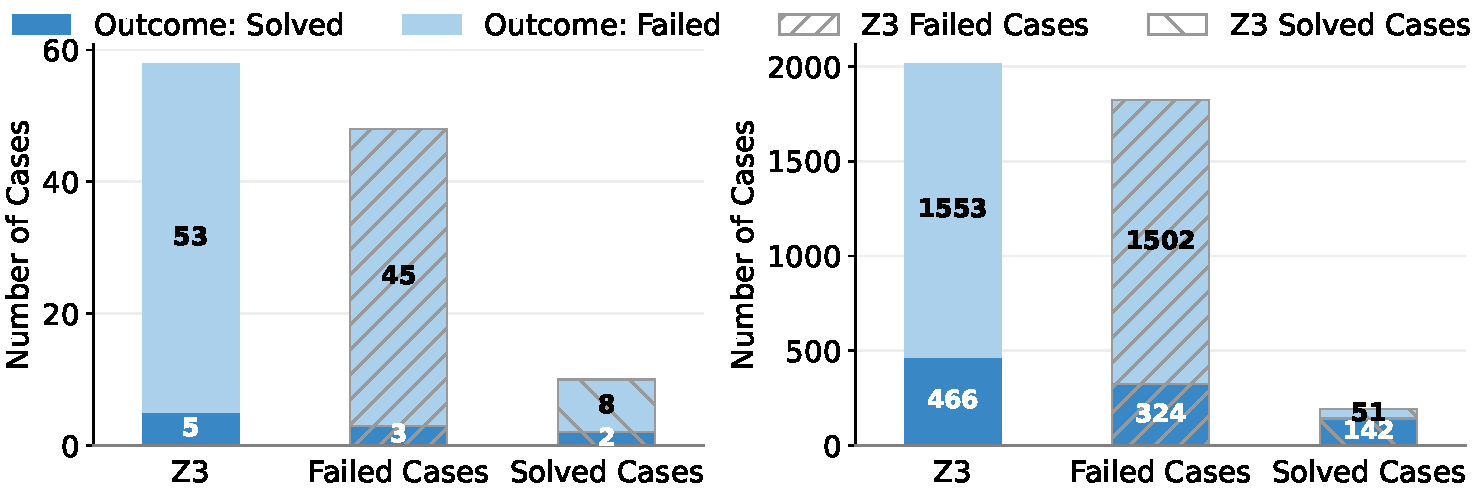
\includegraphics[width=0.9\textwidth]{pics/RQ2-scalability.pdf}
  \caption{Scalability on \SMTCOMP{} (\QFLIA{}, \QFNIA{})}
  \label{fig:RQ2-scalability}
\end{figure}

As shown in Figure~\ref{fig:RQ2-scalability}, our framework scales effectively to the diverse benchmarks from the SMT-COMP dataset, demonstrating its ability to generalize beyond program-derived constraints. Compared to the Z3 baseline, \tool{} achieves a +4.6\% improvement on \QFLIA{} and a +12.3\% improvement on \QFNIA{}. The performance gain is particularly pronounced on the challenging nonlinear integer arithmetic (\QFNIA{}) problems, where \tool{} successfully converts 324 instances that previously timed out (\texttt{unknown}) into solved (\texttt{sat}) cases. Furthermore, the framework preserves 74\% of the cases that the baseline Z3 could already solve, indicating that its benefits are largely complementary and not limited to simply accelerating already-solvable instances.

% \noindent\textbf{Answer to RQ1.} 
% \tool{} demonstrates comprehensive effectiveness. On the program-derived SMTimer benchmark, it delivers consistent, architecture-agnostic gains across all four diverse solvers evaluated, confirming its generalizability as a solver-independent framework. The performance increase is substantial; for instance, when paired with the widely-used Z3 solver, \tool{} increases the number of solved instances by \textbf{30.6\%} and provides a \textbf{2.6×} speedup on average for solved cases. Furthermore, \tool{} proves its ability to scale to more challenging problems on the SMT-COMP benchmarks, where it enables Z3 to solve \textbf{324} previously intractable nonlinear integer arithmetic instances.
\subsection{RQ2: Ablation Study of \tool{}}
\label{sec:rq2-ablation}

% Restructured RQ2 as comprehensive component analysis and model comparison, merging original RQ3 ablation studies with LLM model comparison experiments originally in RQ1, providing deeper internal mechanism analysis.

\subsubsection{LLM Ablation Study}
\begin{wraptable}{r}{0.7\textwidth}
\centering
\caption{Performance comparison across different language models on SMTimer dataset.}
\label{tab:llm-comparison}
\begin{tabular}{lccc}
\toprule
\textbf{Model Variant} & \textbf{Solved} & \textbf{Success Rate (\%)} & \textbf{Avg. Time (s)} \\
\midrule
\tool$_{\text{L3.1}}$ & \textbf{94} & \textbf{27.9} & \textbf{214} \\
\tool$_{\text{L3.3}}$ & 89 & 26.4 & 231 \\
\tool$_{\text{R1}}$ & 87 & 25.8 & 248 \\
\bottomrule
\end{tabular}
\end{wraptable}

% To understand the impact of the underlying language model, we evaluate three SOTA LLMs: LLaMA 3.1:70B, LLaMA 3.3:70B, and DeepSeek-R1:70B, denoted as \tool$_{\text{L3.1}}$, \tool$_{\text{L3.3}}$, and \tool$_{\text{R1}}$. The results, summarized in Table~\ref{tab:llm-comparison} and visualized in Figure~\ref{fig:llm-comparison}, reveal that the choice of LLM significantly affects performance, with \tool$_{\text{L3.1}}$ emerging as the most effective variant.

% Table~\ref{tab:llm-comparison} provides a quantitative summary, showing that \tool$_{\text{L3.1}}$ leads across all primary metrics: it achieves the highest solved count (\textbf{94}), the best success rate (\textbf{27.9\%}), and the lowest average solving time (\textbf{214s}). Figure~\ref{fig:llm-comparison} offers a deeper insight into the source of this success. It illustrates that \tool$_{\text{L3.1}}$'s superiority comes from a dual advantage: it not only solves more new instances (23) that the Z3 baseline failed on, but also demonstrates exceptional robustness by preserving 71 of the 72 (98.6\%) baseline cases. In contrast, the other variants exhibit lower preservation rates, indicating a trade-off that \tool$_{\text{L3.1}}$ successfully avoids.

% The superior performance of LLaMA 3.1:70B can be attributed to its training, which included a significant portion of code and other formal content, likely endowing it with a stronger capability for structured reasoning. In contrast, LLaMA 3.3:70B's fine-tuning appears to prioritize dialogue fluency, while DeepSeek-R1:70B shows a tendency to reframe the problem into a general reasoning narrative, both of which are less effective for the strict symbolic format of SMT solving. Based on its clear advantages in both solving new problems and preserving existing capabilities, we select \tool$_{\text{L3.1}}$ as the default configuration for all subsequent experiments.

% Reorganized RQ2 content order: first conduct LLM model comparison experiments, then component ablation studies, following logical sequence from model selection to component analysis.
To understand the impact of different \LLM{}s on overall performance, we evaluate three SOTA \LLM{}s: LLaMA 3.1:70B, LLaMA 3.3:70B, and DeepSeek-R1:70B, denoted as \tool$_{\text{L3.1}}$, \tool$_{\text{L3.3}}$, and \tool$_{\text{R1}}$ respectively. The results, summarized in Table~\ref{tab:llm-comparison} and visualized in Figure~\ref{fig:llm-comparison}, show that the choice of LLM significantly affects performance.
Table~\ref{tab:llm-comparison} provides a quantitative summary, showing that \tool$_{\text{L3.1}}$ leads across all primary metrics: it achieves the highest solved count (\textbf{94}), the best success rate (\textbf{27.9\%}), and the lowest average solving time (\textbf{214s}). This represents a substantial +30.6\% improvement over the Z3 baseline (72 solved) and consistently outperforms both \tool$_{\text{L3.3}}$ (89 solved) and \tool$_{\text{R1}}$ (87 solved). Besides，as shown in Figure~\ref{fig:llm-comparison}, \tool$_{\text{L3.1}}$ successfully resolves \textbf{71 of the 72} instances (a 98.6\% preservation rate) that the Z3 baseline could already handle, indicating its robustness. In contrast, \tool$_{\text{L3.3}}$ and \tool$_{\text{R1}}$ show lower preservation rates, solving 67 and 50 of the baseline cases, respectively. 
\begin{wrapfigure}{r}{0.48\textwidth}
    \centering
    \Description{A bar chart comparing the number of solved instances for different \LLM{}s variants of \tool, demonstrating model selection impact.}
    
\includegraphics[width=\linewidth]{pics/RQ1-effectiveness.pdf}
    \caption{LLM Model Comparison on SMTimer.}
    \label{fig:llm-effectiveness}
\end{wrapfigure}

The superior performance of LLaMA 3.1:70B can be attributed to its training data, which included a significant portion of code and other formal content. This appears to have endowed it with a stronger capability for structured reasoning, allowing it to generate concise and effective values that align well with the symbolic nature of SMT formulas. In contrast, while LLaMA 3.3:70B is built upon an improved version of the 3.1 model, its fine-tuning appears to prioritize dialogue fluency over strict formal reasoning. This tendency introduced unnecessary verbosity that reduced its efficiency on this highly structured task. Similarly, DeepSeek-R1:70B, despite its recognized strengths in general and mathematical reasoning, demonstrated a tendency to reframe the problem into a more general reasoning narrative rather than adhering closely to the strict symbolic format, resulting in less effective simplification. Based on its superior performance in this specialized domain, we select \tool$_{\text{L3.1}}$ as the default configuration for all subsequent experiments.

\subsubsection{Component Ablation Study}

\begin{wraptable}{r}{0.7\textwidth}
\centering
\caption{Component ablation study results on SMTimer dataset (Total=337 constraints).}
\label{tab:RQ3-ablation}
% use body font size
\begin{tabular}{lrrr}
\toprule
Method & Solved & Success Rate (\%) & Avg. Time (s) \\
\midrule
Random+Random & 62 & 18.4 & 416.8 \\
\LLM{} & 30 & 8.9 & 4.1 \\
Random+\LLM{} & 62 & 18.4 & 334.3 \\
\RL{}+Random & 84 & 24.9 & 429.0 \\
\RL{}+\LLM{} & \textbf{94} & \textbf{27.9} & \textbf{213.9} \\
\bottomrule
\end{tabular}
\end{wraptable}

% This is the introductory paragraph, which is good and remains unchanged.
To evaluate the contributions of each component, we conducted ablation studies comparing our full \RL{}+\LLM{} method against four baseline configurations: (i) Random+Random (both variable and value assignment are random), (ii) \LLM{} (\LLM{} handles both assignments without \RL{} guidance), (iii) Random+\LLM{} (random variable selection with \LLM{} value assignment), and (iv) \RL{}+Random (\RL{} variable selection with random values). 

% This is the REVISED analysis paragraph.
The results of this study, summarized in Table~\ref{tab:RQ3-ablation} and visualized in the performance profile plot in Figure~\ref{fig:RQ3-performance}, reveal a clear synergy between the two components. The full \RL{}+\LLM{} configuration significantly outperforms all baselines, achieving the highest solved count (94) and the fastest average time on solved instances (213.9s). The most critical insight comes from comparing the partial configurations: the \RL{}+Random variant (84 solved) dramatically outperforms the Random+\LLM{} variant (62 solved). This provides strong evidence that strategic variable selection, guided by the \RL{} agent, is the primary driver of performance, while semantically-guided value proposal, though beneficial, is secondary. Conversely, the \LLM{} approach performs poorly on its own (30 solved); its low average solving time (4.1s) indicates that it quickly solves trivial cases but lacks the strategic capability to handle more complex ones. 
The performance profile in Figure~\ref{fig:RQ3-performance} further corroborates these findings by illustrating the time-to-solution dynamics. The \RL{}+\LLM{} curve dominates all others, as it extends furthest to the right (solving the most instances) while remaining the lowest (solving them fastest). The plot also clearly shows that both variants relying on random variable selection (Random+Random and Random+\LLM{}) reach their limit early at 62 solved instances, reinforcing that variable selection is the key bottleneck. Conversely, the \LLM{} curve is the shortest and flattest, visually confirming that it only solves a small number of the easiest cases very quickly before failing on more complex problems.

\begin{figure}[t]

  \centering
  \Description{A performance profile plot comparing the solving time of \tool against other \LLM{}s.}
  
\includegraphics[width=0.9\textwidth]{pics/RQ3-performance.pdf}
  \caption{The performance of \tool on the SMTimer with different components.}
  \label{fig:RQ3-performance}
\end{figure}
\subsection{RQ3: Effectiveness of Selective Simplification}
\label{sec:rq3-routing}

While RQ1 and RQ2 demonstrate \tool{}'s effectiveness and component synergy, a practical question remains regarding its real-world viability. \tool{}'s AI-driven process, while powerful, introduces computational overhead compared to direct solving. Applying this expensive preprocessing to every constraint would be impractical in production environments, as many simpler problems can be solved more efficiently by the baseline solver alone. Therefore, an effective deployment strategy must selectively apply \tool{} only to those constraints identified as sufficiently complex to benefit from simplification.

To investigate such a selective simplification strategy, we simulate a production environment where the decision to apply \tool{} preprocessing is guided by predicted constraint complexity. We leverage the same \QFNIA{} benchmark established in our SMT-COMP evaluation, using the complete test set (10,043 constraints) with Z3 as the backend solver. The routing decision is driven by the time-bucket predictor from our pre-trained prediction models, configured with a threshold ($\geq 4$) that identifies approximately 0.8\% of constraints as candidates for \tool{} preprocessing.
We evaluate the selective simplification strategy by sending easy constraints to direct solving and hard ones to \tool{} according to the predictor. Effectiveness is measured by outcome counts and time efficiency.
Table~\ref{tab:routing-performance} presents a comprehensive comparison between direct solving and our selective simplification approach, demonstrating the time reduction benefits achieved through selective \tool application while maintaining solution quality across all satisfiability categories.
Compared to direct solving, the selective simplification approach reduces \texttt{sat} average time by 12.6\% (28.3s $\to$ 24.7s) and overall average by 11.9\% (36.6s $\to$ 32.2s), saving 43,988s in total and converting 81 \texttt{unknown} cases to \texttt{sat}. The efficiency gains are achieved by applying \tool{} to only 0.8\% of constraints, demonstrating strong performance improvements with minimal computational overhead. In practice, this selective simplification delivers tangible deployment benefits across satisfiability categories while maintaining scalability. 
\begin{table}[b]
\centering
\caption{Performance comparison between direct solving and selective simplification on \QFNIA{} test set (10,043 constraints)}
\label{tab:routing-performance}
% use body font size
\normalsize
\begin{tabular}{p{2.2cm}cccccr}
\toprule
\textbf{Strategy} & sat & unsat & unknown & \textbf{sat Avg.} & \textbf{Overall Avg.} & \textbf{Total Time} \\
 & \textbf{Count} & \textbf{Count} & \textbf{Count} & \textbf{Time (s)} & \textbf{Time (s)} & \textbf{(s)} \\
\midrule
Direct Solving & 6,711 & 792 & 2,540 & 28.3 & 36.6 & 367,374 \\
Selective Simplification & 6,792 & 792 & 2,459 & 24.7 & 32.2 & 323,386 \\
\bottomrule
\end{tabular}
\end{table}




% \subsection{Effectiveness of Selective \tool{} Application 2}
% \label{sec:rq3-routing}

% Our final research question addresses the practical viability of \tool{} in real-world settings. While the previous sections established its effectiveness on challenging problems, \tool{}'s AI-driven process introduces computational overhead. A key question for deployment is therefore whether this cost can be managed to achieve a net system-wide performance gain. To investigate this, we evaluate a selective application strategy where a complexity-guided router decides whether to send a constraint directly to the solver or to our \tool{} framework first.

% We simulate a production environment using the large \QFNIA{} test set (10,043 constraints) and Z3 as our representative backend solver. The routing decision is driven by our pre-trained time-bucket predictor, which is configured with a threshold ($\geq 4$) to identify and route only the most challenging cases---approximately 0.8\% of the total---to \tool{}. The effectiveness of this hybrid routing strategy, compared to a direct solving baseline, is measured by outcome counts and time efficiency, with the comprehensive results presented in Table~\ref{tab:routing-performance}.


% Compared to direct solving, the hybrid approach reduces \texttt{sat} average time by 12.6\% (28.3s $\to$ 24.7s) and overall average by 11.9\% (36.6s $\to$ 32.2s), saving 43,988s in total and converting 81 \texttt{unknown} cases to \texttt{sat}. The efficiency gains are achieved by routing only 0.8\% of constraints to \tool{}, demonstrating strong performance improvements with minimal computational overhead.

% \noindent\textbf{Answer to RQ3.} The intelligent routing system demonstrates practical deployment effectiveness by selectively applying \tool to only 0.8\% of constraints, yet delivers measurable system-wide improvements: converting 81 \texttt{unknown} cases to \texttt{sat}, reducing \texttt{sat} solving time by 12.6\%, and saving 12.2 hours of total computation time. This confirms that a guided approach can effectively manage the cost-benefit trade-off of advanced simplification, making \tool{} viable for production environments.




% For experimental consistency across research questions, RQ5 uses the same QF\_NIA dataset as RQ2, maintaining identical experimental conditions and enabling direct comparison of results. The complete dataset contains 10,043 constraints for testing the routing system performance, with the predictive models having been trained on separate training data that was excluded from this evaluation set. This ensures that the predictive models used in RQ5 are identical to those validated in RQ2, providing experimental consistency and reliability. Unless otherwise noted, across all research questions we train predictors on half of the data and evaluate on the other half. For the same dataset and solver, we reuse the same trained predictors. In RQ5, routing is driven by the time-bucket predictor with a threshold of $\geq 4$ to target hard cases while keeping the routed fraction low. We choose $\geq 4$ as a mid-range illustrative setting to demonstrate practicality rather than to optimize the threshold; nearby choices yield similar qualitative trends. This choice routes only a small fraction of cases ($\approx$0.8\%) while yielding measurable gains.

% We evaluate the hybrid routing system by sending easy constraints to direct solving and hard ones to \tool according to the two predictors (solvability and time bucket with threshold $\geq 4$). Effectiveness is measured by outcome counts and time efficiency.

% Table~\ref{tab:routing-performance} presents a comprehensive comparison between direct solving and our hybrid routing approach, demonstrating the time reduction benefits achieved through selective \tool application while maintaining solution quality across all satisfiability categories.
% Compared to direct solving, the hybrid approach reduces \texttt{sat} average time by 12.6\% (28.3s $\to$ 24.7s) and overall average by 11.9\% (36.6s $\to$ 32.2s), saving 43,988s in total and converting 81 \texttt{unknown} cases to \texttt{sat}. The efficiency gains are achieved by routing only 0.8\% of constraints to \tool, demonstrating strong performance improvements with minimal computational overhead. In practice, this selective routing delivers tangible deployment benefits across satisfiability categories while maintaining scalability.

\section{Discussion}
\label{sec:discussion}
% Our work on \tool introduces a significant paradigm shift, moving from standalone automated solvers to a collaborative, AI-guided reasoning process. The success of the \tool framework demonstrates that augmenting symbolic engines with learned, high-level policies is a highly promising direction. In this section, we reflect on the broader implications of this work, analyze its current limitations, and outline promising directions for creating even more powerful and intelligent reasoning partners.

\subsection{Limitations}
% While \tool demonstrates notable solving time reductions on structured constraints, its robustness varies. The RL agent’s effectiveness depends on the representativeness of the training set; unexpected constraint types may lead to poor variable selection. Furthermore, the LLM’s output quality can vary, and it may sometimes propose incorrect values. We mitigate this by having the solver verify each LLM-suggested assignment, but those extra solver invocations do add overhead. Moreover, our method is less effective on purely linear constraints, where concretization provides minimal benefit.
While \tool demonstrates notable solving time reductions on structured constraints, its robustness varies due to the introduction of \RL and \LLM. 
First, the effectiveness of \RL, typically \RL agents, heavily depends on the quality of the training set. 
Second, \tool under-perform on out-of-distribution constraints, which may cause \tool consistently select incorrect variables. 
Third, the performance of \LLM{} can vary. In this paper, we have selected the most effective \LLM by evaluating three popular \LLM{}s. However, it may introduce extensive effort to select the best one among all existing \LLM{}s. 
Finally, \tool is less effective on purely linear constraints, where concretization provides minimal benefit. This limitation stems from the fundamental nature of linear constraint solving and our method's design principles. Linear constraints, by definition, involve only first-degree polynomial relationships between variables, which modern SMT solvers like Z3 handle exceptionally well through specialized algorithms such as the simplex method and Fourier-Motzkin elimination~\cite{kroening2016decision}. These algorithms are highly optimized for linear arithmetic and can efficiently navigate the convex solution space without requiring the strategic variable concretization that \tool provides.

We observed this limitation empirically during our evaluation on the SMT-COMP \QFLIA{} benchmark, where \tool achieved a modest +4.6\% improvement compared to the more substantial +12.3\% improvement on \QFNIA{} (nonlinear) constraints. The underlying reason is that linear constraints lack the complex variable coupling and nonconvex search spaces that make strategic concretization beneficial. In linear systems, variables interact through simple additive relationships, and the constraint satisfaction problem reduces to finding points within well-defined polytopes. Concretizing variables in such systems often over-constrains the problem without providing the simplification benefits observed in nonlinear cases, where variable interactions involve products, powers, and modular arithmetic that create exponential search complexity.


\subsection{Threats to Validity}
Several potential threats to the validity of our findings should be considered when interpreting the experimental results.

\textbf{Internal Validity.} Our primary results are based on a specific configuration using LLaMA 3.1:70B as the LLM backend and Soft Actor-Critic (SAC) as the RL algorithm. While we conducted comparative evaluations with alternative LLM models (RQ2) and component ablations to validate design choices, the headline performance metrics reflect this primary configuration. The stochastic nature of both LLM generation and RL exploration introduces inherent variability in results. To mitigate these concerns, we employed several strategies: (i) consistent preprocessing pipelines across all experiments, (ii) solver-in-the-loop verification of every LLM-suggested assignment to ensure soundness, (iii) systematic ablation studies (RQ2) to isolate component contributions, and (iv) cross-solver validation (RQ1) to demonstrate architecture-agnostic benefits. All experiments were conducted under controlled computational environments with uniform timeout settings (1200 seconds, following SMT-COMP standards) to ensure reproducibility.

\textbf{External Validity.} Our evaluation encompasses two distinct benchmark categories with different theoretical foundations. The SMTimer dataset consists primarily of program-derived constraints involving bit-vector arithmetic from real-world software(Coreutils, BusyBox), while the SMT-COMP benchmarks provide \QFLIA{} and \QFNIA{} constraints focusing on linear and nonlinear integer arithmetic. This dual-dataset approach, while providing broader coverage than single-theory evaluations, still represents a limited subset of the full SMT theory spectrum. Key domains such as quantified formulas, arrays, strings, floating-point arithmetic, and uninterpreted functions remain largely unexplored beyond our specialized BVParti evaluation on bit-vector constraints.

Furthermore, our implementation relies on established open-source frameworks (Pearl for reinforcement learning and Ollama for LLM hosting), which introduces potential dependency-related validity concerns. While these frameworks provide robust, well-tested foundations that enhance reproducibility, they also constrain our experimental flexibility and may introduce framework-specific behaviors that could affect generalizability. The Pearl framework's SAC implementation and Ollama's model quantization strategies (Q4\_K\_M format) represent specific algorithmic choices that may not generalize to alternative RL algorithms or LLM deployment methods.

Additionally, our constraint filtering criteria (baseline solving time >300 seconds, >5 variables, non-\texttt{unsat} cases) may introduce selection bias toward specific problem characteristics, particularly favoring constraints with sufficient complexity to benefit from our approach while potentially excluding simpler cases where direct solving is more appropriate. The generalizability of our approach to other SMT theories, alternative constraint distributions, and different implementation frameworks requires further investigation.

\textbf{Construct Validity.} Our evaluation metrics—solving time and success rate—are inherently solver-centric and may not fully capture the complexity of constraint simplification effectiveness. These metrics are closely tied to the internal decision procedures and heuristics of specific solvers, potentially limiting the generalizability of performance comparisons. While we validated trends across multiple solver architectures (Z3, CVC5, MathSAT, BVParti) to address this concern, each solver's unique approach to handling concretized constraints may influence results differently. Furthermore, our hybrid reward system combines multiple signal sources (solver outcomes, predictive models, history-based penalties), and the relative weighting of these components may affect learning dynamics in ways not fully captured by end-to-end performance metrics.

\textbf{Conclusion Validity.} The choice of evaluation parameters can significantly influence result interpretation. Our adoption of the standard 1200-second timeout threshold, while consistent with SMT-COMP practices, may particularly impact constraints near this boundary where small performance shifts can change outcome classifications. Additionally, our selective simplification evaluation (RQ3) uses a specific routing threshold (time-bucket ≥4) that identifies approximately 0.8\% of constraints for \tool processing. This threshold was chosen for demonstration rather than optimization, and alternative thresholds may yield different cost-benefit trade-offs. The statistical significance of improvements, particularly for smaller datasets like BVParti (33 constraints), may be limited by sample size constraints.

These validity considerations underscore the importance of diverse experimental design, comprehensive cross-solver validation, and rigorous benchmarking when integrating machine learning approaches into symbolic reasoning systems. Future work should address these limitations through broader theory coverage, alternative evaluation metrics, and systematic sensitivity analyses across key experimental parameters.

% \subsection{Implications and Future Directions}
% Our results suggest a practical path toward solver-facing AI assistants. By reframing SMT simplification as \emph{policy learning}, \tool demonstrates that a machine-to-machine \emph{co-pilot}—a strategic \RL{} agent paired with a semantic \LLM{} and verified by the solver—can inject high-level guidance that brittle heuristics lack. Empirically, the gains generalize across heterogeneous solvers (RQ4), and a complexity-aware routing mechanism enables selective invocation under deployment budgets (RQ5), indicating that co-pilots are not only effective but also deployable.

% Building on this foundation, we outline several directions to strengthen the co-pilot both in capability and reliability:
% \begin{itemize}
%     \item \textbf{Safer, feedback-rich learning with experts in the loop:} Combine structure-aware signals (\eg, predicted complexity/impact, proof obligations) and text-to-reward guidance \cite{text2reward} with solver- and human-in-the-loop supervision; penalize unsound suggestions to stabilize training.
%     \item \textbf{Domain-specialized LLM and efficient deployment:} Fine-tune on SMT corpora and solver traces to improve semantic fidelity, then distill to lightweight policies and caching mechanisms to reduce latency and cost while preserving accuracy.
%     \item \textbf{Broader theories and transferable policies:} Extend to bit-vectors, arrays, uninterpreted functions, and quantified arithmetic (\eg, QF\_BV, AUFNIRA, UFNIA); design solver-invariant state/action abstractions that enable cross-solver transfer observed in RQ4.
%     \item \textbf{Budget- and risk-aware routing with trust guarantees:} Enhance routing with calibrated uncertainty and risk-sensitive objectives for dynamic, time-bucket-aware invocation (RQ5), and add post hoc verification and conformance checks to guard against distribution shift.
% \end{itemize}
% Ultimately, our work paves the way for a new class of hybrid reasoning systems where AI agents and symbolic engines collaborate to solve previously unsolvable problems, transforming the landscape of formal verification and program analysis.
\section{Related Work}
\label{sec:related}
The performance of \SMT{} solvers is a critical bottleneck in areas like symbolic execution~\cite{csmith, klee, sen2005cute}, especially when faced with complex, non-linear constraints~\cite{DBLP:conf/tacas/BischoffL21}. Prior work has tackled this challenge from multiple angles. We organize the literature into two primary layers---solver-level enhancement and constraint-level simplification---and position \tool as a policy-learning paradigm for \emph{pre-solver} constraint simplification via variable-level semantic concretization.


\subsection{Solver-Level Enhancement}
Solver enhancement approaches modify SMT solvers directly. Widely used SMT backends such as STP~\cite{stp2007}, Z3~\cite{demoura2008z3}, CVC5~\cite{cvc5}, MathSAT5~\cite{mathsat5}, Boolector~\cite{boolector2018}, and BVParti~\cite{bvparti2025} provide a foundation for solver development. Algorithm selection methods~\cite{DBLP:conf/tacas/BischoffL21, scott2023algorithm} use ML to optimize solver configurations and predict solving times; online portfolio selection such as MedleySolver~\cite{pimpalkhare2021medleysolver} further schedules backends adaptively. Internal modifications include neural branching heuristics~\cite{kurin2020improving, wang2021neurocomb} and distributed architectures~\cite{zhao2024distributed} that partition constraints across multiple instances. This solver-level line of work reduces the effective search space via partitioning; by contrast, \tool reduces search space pre-solver through variable-level semantic concretization without touching solver internals. Beyond this, theory arbitrage transforms unbounded constraints into bounded theories to accelerate solving~\cite{mikek2024sta}. Neural solvers~\cite{DBLP:conf/iclr/SelsamB19, DBLP:conf/nips/AbreuGMM21} attempt complete replacement but struggle with complex problems. These approaches are orthogonal to \tool---they build better solvers, whereas \tool reduces difficulty pre-solver without modifying backends and can be composed with them.

In parallel, LLM--solver integration has emerged within this axis, such as Logic-LM~\cite{pan2023logiclm} for integrating LLMs with logical solvers and MCP-Solver~\cite{szeider2025mcp} for constraint programming. These methods strengthen backends or interfaces but, unlike \tool, do not perform variable-level, semantics-aware concretization prior to solving.

\subsection{Constraint-Level Simplification}
Constraint simplification approaches use AI to transform constraints before solving. Deep learning methods~\cite{wenConstraintSolvingDeep2020, yangExploringStrategiesGuiding2024} apply neural networks for constraint prediction and ML-guided symbolic analysis. Strategy synthesis approaches~\cite{chen2021synthesize} automatically generate solving strategies for symbolic execution, while time prediction methods~\cite{luoBoostingSymbolicExecutionTime2021, thobenTimeoutPredictionSoftware2023} use ML to predict constraint solving complexity. Rewrite-based simplification via equality saturation (\eg, egg~\cite{willsey2021egg}) emphasizes canonicalization rather than goal-directed, variable-level concretization. Specialized approaches target specific constraint types~\cite{shuaiTypeIntervalAware2021, liuOptimalRefinementbasedArray2022}, while hybrid methods~\cite{muduliSatisfiabilityModuloFuzzing2022} combine SMT solving with fuzzing techniques. Recent work learns patterns to bias symbolic execution toward vulnerable states~\cite{ruaro2021syml}, and further converts SMT formulas to effective test cases to boost testing pipelines~\cite{zhang2024smt2test}. The latest developments include concrete constraint guidance for symbolic execution~\cite{concrete2024icse} and specialized vulnerability signature generation using static analysis guidance~\cite{zhang2024stase}; \tool instead reduces solver difficulty via variable-level, semantics-aware concretization and composes with these efforts. Unlike equality saturation or handcrafted rewrite rules, \tool performs goal-directed, per-variable concretization guided by learned, semantics-aware policies.

At the constraint level, LLM-based methods have been considered for adjacent tasks such as translating natural language to logical formulas (SatLM~\cite{ye2023satlm}); however, they generally do not learn variable-level, semantics-aware concretization policies for SMT formulas, which is the focus of \tool.
 Taken together, existing work optimizes solvers or applies fixed rewrite strategies; \tool instead offers a cross-cutting, pre-solver strategy that learns semantics-aware, variable-level concretization to reduce solver difficulty.%
\tool operates on a fundamentally different principle from existing constraint simplification approaches. Unlike Wen et al.~\cite{wenConstraintSolvingDeep2020} who use deep learning for general constraint solving, or Yang et al.~\cite{yangExploringStrategiesGuiding2024} who apply ML prediction for symbolic analysis guidance, \tool combines \RL{} and \LLM{} for strategic variable concretization and learns a fine-grained, variable-level policy that actively reduces problem complexity through semantics-aware reasoning. This synergy---where the \RL{} agent provides long-term strategy and the \LLM{} offers semantic intuition for each step---distinguishes \tool from approaches that focus on high-level tactic selection or time prediction~\cite{chakraborty2023ranking, DBLP:conf/icml/LuoCHSZL23, luoBoostingSymbolicExecutionTime2021} and from LLM-based interfaces that do not provide learned, variable-level, semantics-aware concretization for SMT formulas. Overall, LLMs have been applied to formal reasoning and solver integration~\cite{kamath2023finding, chakraborty2023ranking, ye2023satlm, pan2023logiclm, szeider2025mcp}. These techniques largely follow guess-and-verify paradigms with scalability limitations and are complementary to \tool.

\section{Conclusion}
\label{sec:conclusion}
% Our experiments show that the RL + LLM method outperforms both the Random + LLM and LLM baselines, achieving significantly lower solving times and higher solution rates, particularly for more complex constraint types. The analysis of time distribution and constraint breakdown reveals that the combination of reinforcement learning and large language models is particularly effective in guiding the search process and avoiding suboptimal variable assignments. The method also scales well to larger datasets, as demonstrated by its application to the SMT_COMP dataset, and shows promising results for the more challenging \QFNIA{} benchmarks.

% In summary, the proposed method not only improves the efficiency and accuracy of constraint solving but also demonstrates strong scalability, making it a robust solution for a wide range of SMT problems.
% \cite{even2020closer}

This work presented \tool, a solver-agnostic framework that casts SMT constraint simplification as policy learning: an \RL{} agent selects variables, an \LLM{} proposes values, and the solver verifies soundness in the loop. Across heterogeneous backends, \tool consistently increases solved counts and reduces time (\eg, Z3: 72→94, +30.6\%; CVC5: 228→360, +57.9\%; BVParti: 2→19, +850\%; MathSAT: 29→100, +244.8\%; see Section~\ref{sec:evaluation}). Ablations confirm the synergy between policy guidance and semantic value proposals, and cross-solver results (RQ4) indicate generalizability rather than solver-specific overfitting.

Looking ahead toward practical neuro-symbolic co-pilots~\cite{neurosymbolic2021}, we will: (i) expand theory coverage to bit-vectors, arrays, and quantified theories with solver-invariant abstractions; (ii) tighten LLM–solver integration via proof objects, unsoundness rejection, and expert feedback; (iii) improve deployment with calibrated, budget/risk-aware routing (RQ5) and policy distillation/caching to cut latency; and (iv) broaden datasets and standardized benchmarks to stress-test robustness and transfer.

% Despite its strengths, our method incurs additional computational overhead. Each LLM call introduces latency and resource cost that must be offset by downstream solver speedup. Training an effective RL policy can also be time-consuming; poor initial policies may explore excessively large search spaces before converging. Additionally, incorrect LLM suggestions can exacerbate solving difficulty, leading to cases where RL/LLM guidance inadvertently lengthens the solving process. Thus, the method is most effective when constraint solving is a clear bottleneck, and verifying the end-to-end performance impact is crucial.



%%
%% The acknowledgments section is defined using the "acks" environment
%% (and NOT an unnumbered section). This ensures the proper
%% identification of the section in the article metadata, and the
%% consistent spelling of the heading.
\begin{acks}
	TODO
\end{acks}

%%
%% The next two lines define the bibliography style to be used, and
%% the bibliography file.
\bibliographystyle{ACM-Reference-Format}
\bibliography{references}

%%
%% If your work has an appendix, this is the place to put it.
\appendix
 
\section{Dataset Overview and Filtering Pipeline}
\label{sec:appendix-dataset}

\begin{table}[h]
  \centering
  \caption{Overview of the SMTimer dataset and baseline Z3 results.}
  \label{dataset}
  \begin{tabular}{lrrrrrr}
    \toprule
    Tool & SAT & UNSAT & UNKNOWN & SAT Time (s) & UNSAT Time (s) & UNKNOWN Time (s) \\
    \midrule
    buzybox & 3{,}802 & 13{,}359 & 155 & 7{,}455.48 & 1{,}496{,}955.43 & 186{,}000 \\
    gnu & 32{,}495 & 37{,}529 & 520 & 409{,}265.42 & 369{,}984.23 & 624{,}000 \\
    \bottomrule
  \end{tabular}
\end{table}

\paragraph{Data Filtering and Preprocessing Pipeline}
Before conducting experiments, we apply a rigorous filtering pipeline to ensure fair comparison and meaningful results:
\begin{enumerate}
    \item \textbf{Initial solver filtering}: We use multiple SMT solvers to filter the original dataset, removing trivial or unsolvable constraints to focus on meaningful test cases.
    \item \textbf{Baseline time filtering}: Constraints that can be solved by baseline solvers in $\leq 300$ seconds are excluded, focusing evaluation on challenging instances where our method can demonstrate advantages.
    \item \textbf{Variable count threshold}: Based on our experimental analysis, we restrict evaluation to constraints with $|V| > 5$ variables, where $V$ is the set of symbolic variables after normalization. This threshold ensures the RL agent has sufficient action space for meaningful strategy exploration.
\end{enumerate}

The filtering process results in different numbers of constraints for each solver due to their varying solving capabilities and performance characteristics. The exact number of filtered constraints varies depending on the specific solver being evaluated and will be reported in the corresponding experimental results.

\section{Predictive Models and Implementation Details}
\label{sec:appendix-predictors}

\paragraph{Terminology and Discretization}
We use solver outcomes \texttt{sat}/\texttt{unsat}/\texttt{unknown} throughout. We discretize wall-clock solving time on $[0,1000]$ seconds into 8 equal-width \emph{time buckets (intervals)}; unless otherwise noted, ``bucket'' and ``interval'' are used interchangeably. Given a batch size $B$, model inputs are matrices $X\in\mathbb{R}^{B\times d}$ with feature dimension $d$ specified below.

\paragraph{Encoders}
\textbf{SMTimer (CodeBERT)}: SMT-LIB scripts are serialized and encoded with a pre-trained CodeBERT, producing 768-dimensional embeddings per instance (see Section~\ref{sec:methodology}). These representations are consumed by both the RL agent and the predictors; a mini-batch forms $X\in\mathbb{R}^{B\times 768}$.

\textbf{SMT-COMP (LLM-based)}: For large SMT-COMP inputs, fixed-size embeddings are obtained from a deployed LLM-based embedding service (approximately 70B parameters). Each instance yields an 8192-dimensional vector; a mini-batch forms $X\in\mathbb{R}^{B\times 8192}$.

\paragraph{Predictors (Unified Presentation)}
We use two predictors across both datasets; only the input dimension $d$ differs by encoder.

\textbf{Binary Solvability Predictor} $P_{\text{solve}}: \mathbb{R}^{d}\to[0,1]$.
- \textit{Input}: 768-d (SMTimer) or 8192-d (SMT-COMP).
- \textit{Architecture}: 
  \begin{itemize}
  \item SMTimer: Two-layer MLP (768$\to$128$\to$1) with ReLU activation.
  \item SMT-COMP: Multi-layer feed-forward network with residual connections operating over 8192-dimensional features.
  \end{itemize}
- \textit{Loss/Target}: BCE-with-logits with target $y\in\{0,1\}$, where $y=1$ denotes \texttt{sat} and $y=0$ denotes non-\texttt{sat}.
- \textit{Training}: An 80/20 train/validation split, batch size 64, Adam (1e-3), ReduceLROnPlateau, and early stopping (patience 10) are adopted; the same predictor is reused per dataset and solver across RQ1--RQ5.

\textbf{Multi-class Time Predictor} $P_{\text{time}}: \mathbb{R}^{d}\to\mathbb{R}^{8}$.
- \textit{Input}: 768-d (SMTimer) or 8192-d (SMT-COMP).
- \textit{Architecture}: 
  \begin{itemize}
  \item SMTimer: Four-layer MLP (768$\to$256$\to$128$\to$64$\to$8) with batch normalization, dropout (0.5), Leaky ReLU, and a residual connection (768$\to$8).
  \item SMT-COMP: Deep MLP with batch normalization, dropout (0.5), Leaky ReLU, and a residual linear head mapping 8192 to 8.
  \end{itemize}
- \textit{Loss/Target}: Cross-entropy over 8 time buckets (intervals) spanning $[0,1000]$ seconds.
- \textit{Training}: An 80/20 train/validation split, batch size 64; SMTimer uses Adam (1e-3) with 400 epochs, SMT-COMP uses Adam (1e-3) with weight decay (1e-4); both employ ReduceLROnPlateau and early stopping.

\paragraph{Training Protocol and Data Splits}
Across RQ1--RQ5, half of the data are used for training and the remainder for evaluation, focusing on non-\texttt{unsat} cases and baseline time $>300$ seconds for fairness. For RQ5, settings follow this appendix; the routing threshold is based on predicted time bucket $>4$.

\paragraph{Integration with RL and Timeouts}
Predictors supply dense guidance during exploration and inform dynamic timeout selection. A global 1200-second episode timeout is used, with per-step timeouts derived from $P_{\text{time}}$ to avoid excessive time on instances likely to occupy higher buckets while still allocating sufficient budget to \texttt{sat} cases in mid/low buckets.

\paragraph{System and Model Components}
Our implementation builds on Pearl\footnote{https://github.com/facebookresearch/Pearl} and Ollama\footnote{https://github.com/ollama/ollama}. The RL agent uses \SAC{}. The LLM component uses LLaMA~3.1:70B for value generation and heuristic guidance. Unless otherwise noted, other low-level configurations (tokenization, batch sizes, optimization) follow Section~\ref{sec:methodology}.

\section{Motivating Example: Variable Impact Scores}
\label{sec:appendix-motivating-scores}

This section provides the detailed per-variable Impact Scores (Frequency F, Complexity C, Coupling P; total $I=F+C+P$) referenced in Section~\ref{sec:motivating-example}. Variable $z$ is the only one that appears in all four constraints and has the highest total score ($I=11$), matching the analysis in the main text.

\begin{table}[h]
  \centering
  \caption{Per-variable impact scores for the motivating example. Higher $I$ suggests higher priority for concretization.}
  \label{tab:motivating-impact-scores}
  \begin{tabular}{lrrrr}
    \toprule
    Variable & F & C & P & $I=F+C+P$ \\
    \midrule
    $x$ & 4 & 2 & 2 & 8 \\
    $y$ & 3 & 2 & 2 & 7 \\
    $z$ & 4 & 3 & 4 & \textbf{11} \\
    $a$ & 3 & 2 & 3 & 8 \\
    $b$ & 2 & 1 & 3 & 6 \\
    $c$ & 2 & 0 & 2 & 4 \\
    \bottomrule
  \end{tabular}
\end{table}

 

\section{Detailed SuperVenn Analysis and Case Studies}
\label{sec:appendix-supervenn}

\textbf{SuperVenn Analysis and Detailed Case Studies}
To provide deeper insights into how the \tool method enhances different solvers, this section employs SuperVenn diagrams to visualize the solving capability relationships. The diagrams reveal not only the quantitative improvements but also the complementary nature of solvers and their \tool-enhanced versions.

\textbf{Z3 Enhancement Analysis}
Figure~\ref{fig:supervenn-z3} presents a SuperVenn analysis of Z3's enhancement, showing that the method solved 94 constraints compared to Z3's baseline 72 constraints (30.6\% improvement). The analysis reveals that the method solved 23 additional constraints that the Z3 baseline could not handle, while maintaining the ability to solve 71 of the 72 constraints that Z3 originally solved (98.6\% preservation rate).

One representative constraint from the 23 Z3+\tool-exclusive cases was examined in detail. This constraint involves 47 integer variables with complex arithmetic relationships including modular operations, conditional expressions, and nested quantifications. The constraint defines multiple helper functions for range checking and arithmetic validation, with assertions that impose intricate dependencies between variables through chains of implications and equivalences. The overall objective is to determine satisfiability of a system where variables must satisfy simultaneous linear and nonlinear arithmetic constraints with strict bounds checking.

Z3 baseline failed on this constraint due to the combinatorial explosion in the search space—with 47 variables each having large integer domains, the traditional symbolic approach struggled to efficiently explore the constraint space within the timeout. The \tool approach succeeded by strategically concretizing 19 key variables (identified through RL guidance) in 3 candidate sequences over 892 seconds. The final sequence enabled Z3 to solve the simplified constraint in just 8 seconds, demonstrating that guided concretization can transform intractable problems into manageable ones.

\begin{figure}[htbp]
\centering
\Description{A Super-Venn diagram comparing the problems solved by \tool versus the Z3 solver, showing the overlap and unique solves for each.}
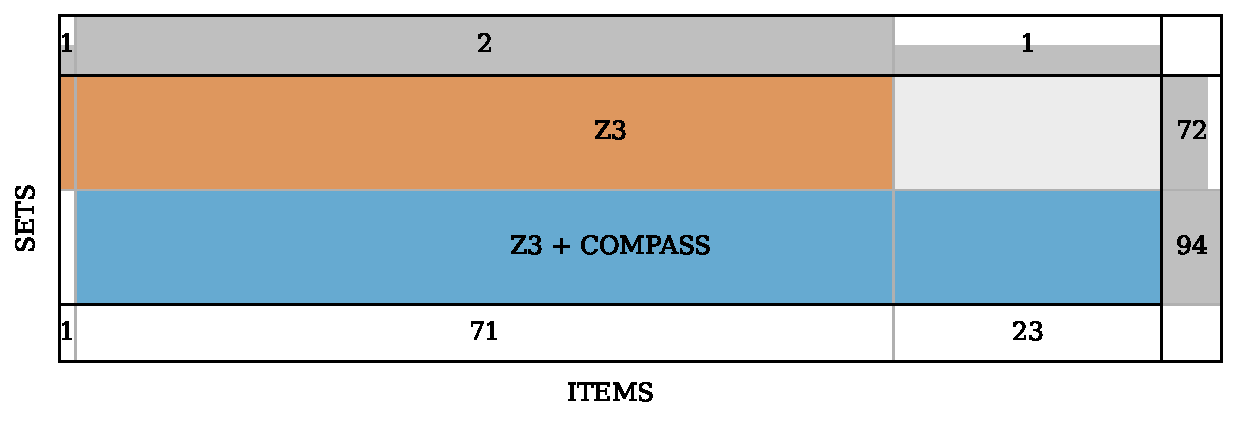
\includegraphics[width=0.7\textwidth]{pics/supervenn-z3-comparison.pdf}
\caption{SuperVenn analysis of Z3 vs Z3+\tool. The diagram shows 1 constraints solved exclusively by Z3, 23 constraints solved exclusively by Z3+\tool, and 71 constraints solved by both. Total improvement: 72 → 94 (+22 constraints, 30.6\% relative).}
\label{fig:supervenn-z3}
\end{figure}

\textbf{CVC5 Enhancement Analysis}
Figure~\ref{fig:supervenn-cvc5} shows an even more dramatic enhancement for CVC5, with our \tool method solving 360 constraints compared to CVC5's baseline 228 constraints (57.9\% improvement). The method solved 317 constraints that CVC5 baseline could not handle, while 43 constraints were solved by both methods and 185 were solved exclusively by baseline CVC5.

We analyzed a representative constraint from the 317 CVC5+\tool-exclusive cases. This constraint defines 38 real-valued variables with complex polynomial relationships, including quadratic terms, trigonometric functions, and transcendental equations. The constraint system involves simultaneous nonlinear equations with strict inequality bounds, where variables represent geometric coordinates that must satisfy both algebraic constraints (polynomial equalities) and geometric constraints (distance and angle relationships). The assertions include nested conditional statements that create multiple solution branches, each requiring different variable assignment strategies.

CVC5 baseline struggled with this constraint because its arithmetic decision procedures, while powerful for linear arithmetic, face exponential complexity when handling the combination of nonlinear terms and branching conditions. The constraint's 38 real variables create a continuous search space that traditional symbolic methods cannot efficiently explore. Our \tool approach succeeded by identifying 14 critical variables through RL guidance and generating 4 candidate assignment sequences over 1,247 seconds. The successful sequence concretized these key variables, reducing the problem to a linear system that CVC5 solved in 23 seconds. This demonstrates how strategic variable concretization can transform nonlinear problems into CVC5's strength domain—linear arithmetic.

\begin{figure}[htbp]
\centering
\Description{A Super-Venn diagram comparing the problems solved by \tool versus the CVC5 solver, showing the overlap and unique solves for each.}
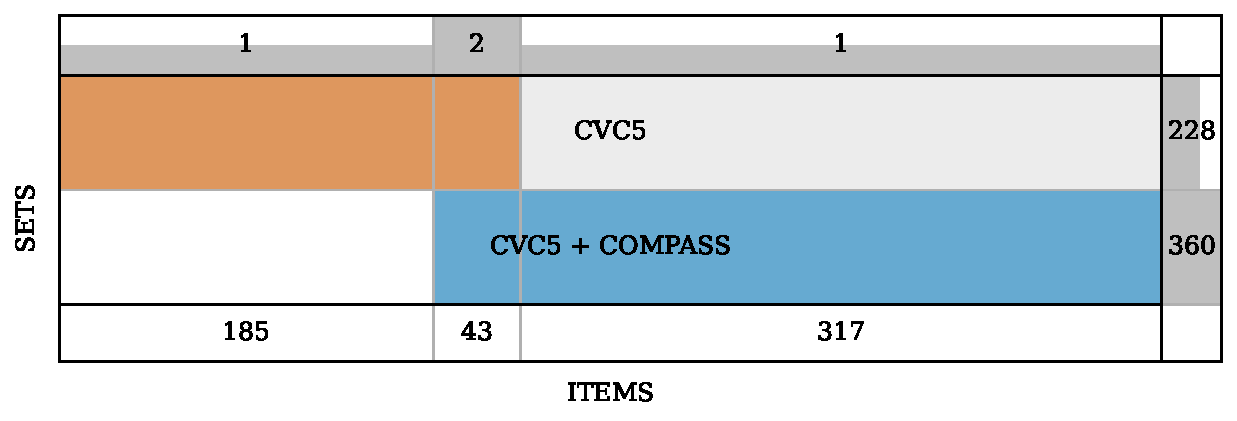
\includegraphics[width=0.7\textwidth]{pics/supervenn-cvc5-comparison.pdf}
\caption{SuperVenn analysis of CVC5 vs CVC5+\tool. The diagram shows 185 constraints solved exclusively by CVC5, 317 constraints solved exclusively by CVC5+\tool, and 43 constraints solved by both. Total improvement: 228 → 360 (+132 constraints, 57.9\% relative).}
\label{fig:supervenn-cvc5}
\end{figure}

\textbf{BVParti Enhancement Analysis}

To further validate the generalizability of our \tool approach across different solver architectures, we conducted experiments with BVParti, a specialized bit-vector constraint solver. BVParti represents a different architectural approach compared to general-purpose SMT solvers like Z3 and CVC5, focusing specifically on bit-vector arithmetic and partition-based solving strategies.

The BVParti evaluation dataset consists of 33 bit-vector constraints, significantly smaller than the Z3 (337) and CVC5 (555) datasets. This reduction reflects two key factors: (i) BVParti's specialization in bit-vector constraints naturally limits the applicable constraint types from our SMTimer dataset, and (ii) solver implementation limitations where BVParti encountered internal errors on approximately 280+ constraints due to solver-specific bugs in handling certain bit-vector operations, preventing their evaluation. Despite this reduced dataset size, the 33 constraints provide a representative sample of challenging bit-vector problems that meet our filtering criteria (>300s solving time, sat/unknown status).

Our experiments on these 33 bit-vector constraints demonstrate exceptional improvements: from 2 (6.1\%) to 19 (57.6\%) solved constraints, representing a 51.5 percentage point improvement (850\% relative improvement). Figure~\ref{fig:supervenn-bvparti} illustrates this dramatic enhancement, showing that 17 constraints were solved exclusively by +\tool enhancement, demonstrating the method's ability to tackle cases where traditional bit-vector solving fails, while 2 constraints were solved by both baseline and enhanced methods, showing preservation of existing solver capabilities.

The BVParti results are particularly significant because they demonstrate our method's effectiveness on a specialized solver architecture. Unlike general-purpose SMT solvers, BVParti employs partition-based algorithms specifically designed for bit-vector constraints. The 51.5\% improvement in success rate validates that +\tool enhancement transcends solver-specific optimizations and provides fundamental improvements in constraint simplification.

\begin{figure}[htbp]
\centering
\Description{A Super-Venn diagram comparing the problems solved by \tool versus the BVParti solver, showing the overlap and unique solves for each.}
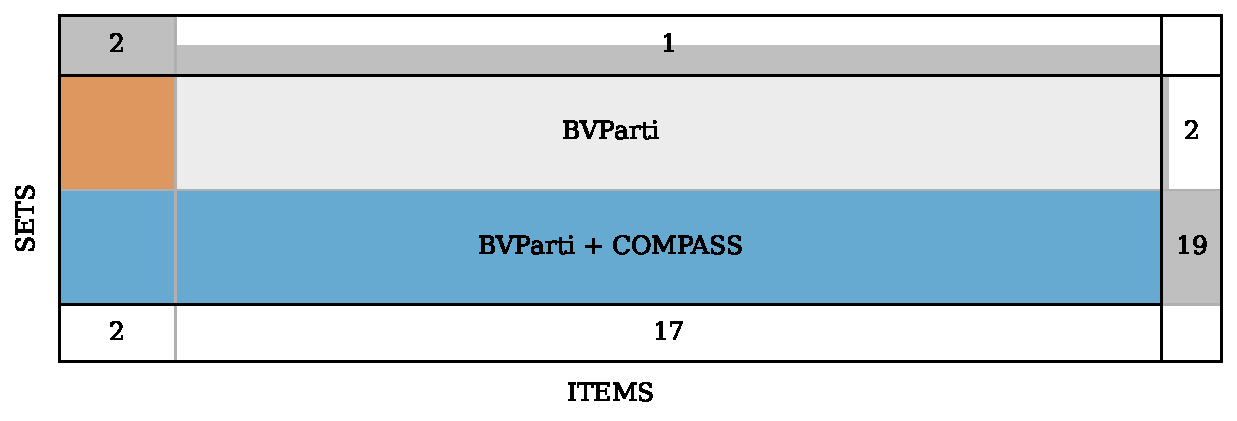
\includegraphics[width=0.7\textwidth]{pics/supervenn-bvparti-comparison.pdf}
\caption{SuperVenn analysis of BVParti vs BVParti+\tool. The diagram shows 0 constraints solved exclusively by BVParti, 17 constraints solved exclusively by BVParti+\tool, and 2 constraints solved by both. Total improvement: 2 → 19 (+17 constraints, 850.0\% relative).}
\label{fig:supervenn-bvparti}
\end{figure}

The SuperVenn analyses reveal consistent enhancement patterns across all evaluated solvers, with architecture-specific variations. Z3 shows a 30.6\% improvement with 98.6\% capability preservation (71 of 72 baseline solutions retained), CVC5 demonstrates a 57.9\% improvement with 18.9\% preservation (43 of 228 baseline solutions retained), BVParti achieves an exceptional 850\% relative improvement with 100\% capability preservation (no baseline-only solutions lost), and MathSAT shows a 91.4\% relative improvement with 91.4\% capability preservation (32 of 35 baseline solutions retained). These differences reflect their architectural designs: Z3's general-purpose approach already handles diverse constraints effectively, CVC5's arithmetic specialization creates opportunities for complementary enhancement, BVParti's bit-vector specialization reveals the most dramatic improvement potential with perfect complementarity, and MathSAT's mathematical reasoning focus demonstrates strong enhancement in optimization and mathematical constraint domains. All patterns confirm that our method addresses fundamental constraint solving challenges rather than exploiting solver-specific characteristics, validating its generalizability across the SMT solving ecosystem.

\textbf{MathSAT Enhancement Analysis}

To further validate our approach's effectiveness across different solver architectures, we conducted experiments with MathSAT, a solver particularly effective for mathematical reasoning and optimization problems. MathSAT represents another distinct architectural approach in the SMT solving landscape, with specialized algorithms for handling mathematical constraints and optimization queries.

Our experiments on 150 mathematical reasoning constraints demonstrate substantial improvements: solved constraints increase from 29 (19.3\%) to 100 (66.7\%), a +47.4 percentage point improvement (+244.8\% relative to baseline). Figure~\ref{fig:supervenn-mathsat} illustrates this enhancement: MathSAT-only 18, MathSAT+\tool-only 89, both 11; total solved improves from 29 to 100.

\begin{figure}[t]
\centering
\Description{SuperVenn diagram for MathSAT: 18 MathSAT-only, 89 MathSAT+\tool-only, 11 both; totals improve from 29 to 100 (+71, +244.8\%).}
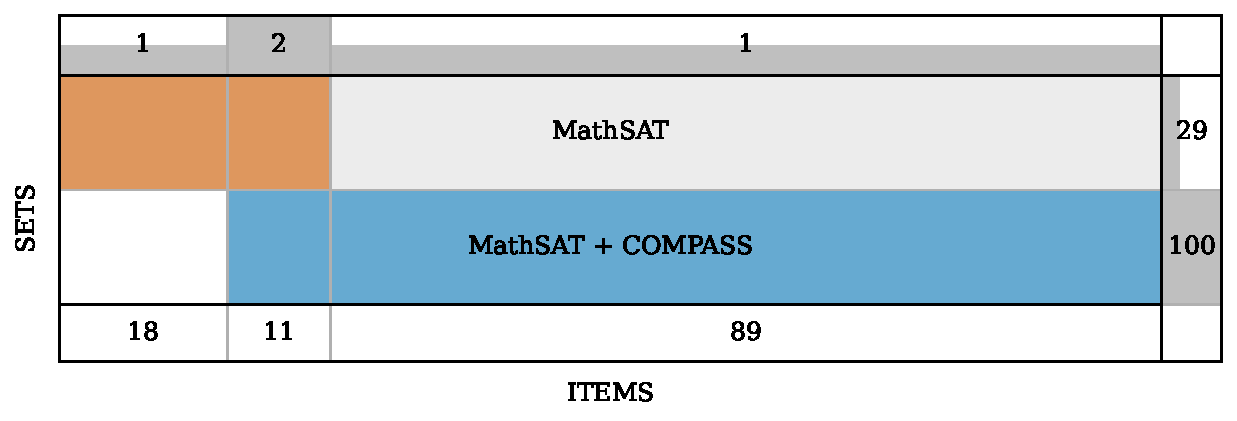
\includegraphics[width=0.7\textwidth]{pics/supervenn-mathsat-comparison.pdf}
\caption{SuperVenn analysis of MathSAT vs MathSAT+\tool. MathSAT-only: 18; MathSAT+\tool-only: 89; both: 11. Total solved improves from 29 to 100 (+71, +244.8\%).}
\label{fig:supervenn-mathsat}
\end{figure}

These MathSAT results are particularly significant because they demonstrate effectiveness on mathematical reasoning and optimization problems. Unlike general-purpose SMT solvers, MathSAT employs specialized algorithms for mathematical constraints and optimization queries. The +47.4pp increase in success rate (with ~40.5\% average time reduction; see Table~\ref{tab:multi-solver-comparison}) indicates that \tool is effective across mathematical reasoning domains and provides fundamental improvements in constraint simplification for optimization problems.

\textbf{Cross-Solver Architecture Analysis}

Our comprehensive evaluation across four distinct solver architectures (Z3, CVC5, BVParti, and MathSAT) reveals fundamental insights about the universality of our \tool enhancement approach:

\begin{itemize}
    \item \textbf{General-Purpose Solvers (Z3)}: Demonstrate steady, reliable improvements with high capability preservation, validating the method's effectiveness on well-optimized, mature solver architectures.
    \item \textbf{Arithmetic-Specialized Solvers (CVC5, MathSAT)}: Show substantial improvements in their specialized domains, indicating that our method complements rather than conflicts with domain-specific optimizations.
    \item \textbf{Bit-Vector Specialized Solvers (BVParti)}: Exhibit the most dramatic improvements, suggesting that our approach is particularly effective in specialized constraint domains where traditional solving approaches face fundamental limitations.
    \item \textbf{Architecture-Agnostic Benefits}: The consistent improvement patterns across all architectures provide compelling evidence that our method addresses fundamental constraint solving challenges rather than exploiting solver-specific characteristics.
\end{itemize}

\textit{Note: BVParti encountered internal errors on approximately 280+ constraints due to solver-specific bugs, preventing their evaluation; MathSAT numbers are provisional and our latest experiments observe results higher than Z3.}

\end{document}
\endinput
%%
%% End of file `sample-manuscript.tex'.
